\chapter{Linguaggi per l'orchestrazione}

Questo capitolo offre una panoramica ad alto livello di BPEL, il
linguaggio che è diventato lo standard per l'orchestrazione dei Servizi Web.
Successivamente viene introdotto Blite, una variante semplificata di
BPEL, che ne riproduce alcune delle funzionalità più caratteristiche al fine
di definire una sematica formale. Tale sematica è presentata e commentata in
dettaglio nella Sezione 2.2. Dalla sintassi astratta di Blite si ricava una
grammatica in notazione EBNF utilizzata dopo per lo sviluppo di un compilatore,
tale procedimento è presentato nella Sezione 2.3.

\section{BPEL: uno standard per l'orchestrazione di Servizi Web}
Abbiamo detto come SOA e i Servizi Web siano una delle risposte più recenti
alla necessità di integrare funzionalità applicative eterogenee, e di fornire
un modello di sviluppo software che sia il pi\`u efficace possibile rispetto
alla natura dinamica dei domini applicativi tipici delle grandi realtà
aziendali.

Alla base della metodologia SOA vi è l'approccio ``bottom-up'', secondo cui è
possibile comporre le funzionalità di base offerte dalle diverse applicazioni
aziendali per crearne di più complesse e articolate. Gli standard e i linguaggi
dei Servizi Web foniscono il supporto tecnologico e formale per realizzare tale
integrazione che nella maggior parte degli scenari reali prevede di dover far
comunicare tecnologie e formalismi del tutto eterogeni e incompatibli. Una delle
possibilità più interessanti è quella di poter utilizzare il patrimonio storico
(``legacy'') del software aziendale tramite standard moderni e aperti, e poter
fare dialogare le applicazioni di ultima generazione con quelle più ``mature'',
che spesso mantengono un alto valore aziendale ma si basano su tecnologie e
metodologie proprietarie ormai difficilmente manutenibili.

Predisporre i componenti e renderli disponibili secondo il paradigma dell'
Architettura Orientata ai Servizi certo non realizza tutte le necessità di un
complesso sistema aziendale, il passo successivo non può essere che quello di
comporre le singole funzionalità di base per realizare i flussi operativi che
implemetano le reali politiche e strategie di business. Le attività aziendali
quindi possono essere rappresentate come processi (``Business Process'') che
raggruppano le singole funzionalità secondo precise regole aziendali (``Business
Rules'') e tramite primitive di aggregazione che attuano dipendenze temporali e
logiche fra i diversi componenti pubblicati come servizi (``Service
Orchestration''). Se si può pensare che le singole funzionalità siano i mattoni
del business e che abbiano una certa robustezza temporale, in termini di
specifica e implemetazione, i processi al contrario possono essere fortemente
dinamici e mutevoli, per poter facilmente adeguarsi alle necessità sempre nuove
che si presentano nelle attività di un'azienda.

Si capisce quindi come nasca la necessità di un formalismo specifico per la
definizione e realizzazione di tali processi. In generale si vorrebe poter
disporre di un linguaggio semplice e flessibile che possa essere utilizzato a
diversi livelli aziendali, compreso e adoperato dalle diverse figure
professionali che partecipano alla definizione e attuazione dei processi
stessi. Si vorrebbe disporre non solo di un linguaggio di programmazione
utile ai tecnici del software ma anche di un formalismo utilizzabile dai manager
e dagli esperti dei domini applicativi, che possa realizzare una piattaforma
comune per la collaborazione fra le diverse aree disciplinari.

\`E proprio come risposta a tale necessità che si propone BPEL, un linguaggio
basato su XML per la definizione di processi aziendali realizzati come
composizione di funzionalità esposte da Servizi Web. BPEL storicamente nasce
dalla fusione di due tecnologie sviluppate indipendetemente all'inizio degli
anni 2000: WSFL (Web Service Flow Language) di IBM \cite{WSFL} e XLANG di
Microsoft \cite{XLANG}. La prima versione del linguaggio (BPEL4WS ``Business
Process Execution Language for Web Services - Version 1.0'' \cite{BPEL10Spec}) risale al 31 Luglio 2002 e
fu prodotta dal lavoro congiunto di grandi aziende come IBM, BEA, SAP, Siebel e Microsoft. Dall'Aprile del 2003 il lavoro
di stesura della versione successiva (1.1 \cite{BPEL11Spec})  è stato affidato
alla supervisione di Oasis \cite{OASISSite}, società nata con il compito di
realizzare standard aperti e condivisi dalla comunità internazionale; al 5
Maggio 2003 è datato il rilascio di questa versione nella stesura ufficiale. Oasis è  anche la curatrice della
versione 2.0 dello standard (WS-BPEL ``Web Services Business Process Execution
Language Version 2.0'' \cite{BPEL20Spec}) che ha visto il primo rilascio
ufficiale in data 11 Aprile 2007.
\\

BPEL, come molti linguaggi legati alla tecnologia dei servizi web, ha una
sintassi basata su XML. Tramite tale sintassi è possibile descrivere un business
process definendo una logica di orchestrazione che determina le elaborazioni
interne e le interazioni con i partner del processo, le quali sono, in entrambi
i casi prodotte dall’esecuzione di attività definite sintatticamente in forma di
tag XML.

In BPEL possono essere date definizioni di processi \emph{eseguibili}, le quali
comprendono  tutti i dettagli relativi ai meccanismi interni del processo e
descrivono in maniera completa l’orchestrazione dei servizi web partner; 
processi di questo tipo possono essere eseguiti da un motore di esecuzione BPEL. 
BPEL permette anche di definire processi \emph{astratti}, che costituiscono una
descrizione del flusso di informazioni tra i partner ed il processo e non
specificano i dettagli delle elaborazioni interne al processo; un processo
di questo tipo non può essere eseguito, poiché mancano i dettagli relativi     
all'orchestrazione, e descrive piuttosto una coreografia di messaggi.
Noi siamo interessati alla descrizione completa dell'orchestrazione di un
insieme di servizi web pertanto
prenderemo in considerazione solo i processi eseguibili.

La definizione di un processo BPEL include la definizione delle relazioni tra
il processo ed i suoi partner, rappresentate dai cosiddetti partner link. Tra le
definizioni WSDL utilizzate dal processo devono essere presenti le definizioni
di uno o più partner link type, espresse tramite uno o più elementi della
forma:

\begin{verbatim}
<partnerLinkType name="ncname">
   <role name="ncname">
      <portType name="qname"/>
   </role>
   <role name="ncname">?
      <portType name="qname"/>
   </role>
</partnerLinkType> 
\end{verbatim}

Ad ogni partner link type viene associato un nome e due \emph{ruoli}, ognuno dei
quali rappresenta una delle due estremità del link ed indica la specifica 
interfaccia (port type) WSDL che deve essere implementata dall'entità posta a
a tale estremità (il processo o uno dei suoi partner). Nel caso in cui uno dei
due ruoli usufruisce delle operazioni dell’altro senza che ad esso sia richiesto
di fornire specifici servizi, viene indicato un solo elemento \texttt{<role>}
(quello relativo all’estremità a cui sono richieste funzionalità specifiche).
Sottolineiamo che  la definizione dei partner link type deve essere contenuta
in un documento WSDL. Di fatto i partner link type a due ruoli introducono la
novità rispetto a WSDL e servono ad estendere il concetto di
\emph{contratto} un una comunicazione asincrona in cui il richidente del
servizio può essere non noto in fase di sviluppo del provider.

La definizione del processo BPEL invece contiene le definizioni dei partner
link veri e propri, espresse da uno o più elementi \texttt{<partnerLink>}
annidati nell’elemento \texttt{<partnerLinks>}:

\begin{verbatim}
<partnerLinks>
   <partnerLink name="ncname" partnerLinkType="qname"
                myRole="ncname"? partnerRole="ncname"?>+
   </partnerLink>
</partnerLinks>
\end{verbatim}

Ciascun partner link viene definito indicando il nome del partner link type e
indicando quali sono il ruolo del processo (tramite l'attributo myRole) ed il
ruolo del partner (tramite l’attributo partnerRole).


Una caratteristica importante di BPEL è la possibilità di utilizzare delle
strutture dati particolari, dette \emph{endpoint reference}, che rappresentano
l'indirizzo fisico di un partner del processo. Gli endpoint reference possono
essere copiati da una variabile ad un'altra oppure possono essere inviati
all'interno dei messaggi trasmessi tra processo e partner; ciò permette di
determinare gli indirizzi fisici degli stessi partner in modo dinamico, durante il corso
dell'esecuzione del processo.

In questo modo un processo BPEL non deve per forza conoscere
fin dall'inizio i suoi partner effettivi, e come precedentemente fatto notare
la cambinazione endpoint reference con i partner link type bidirezionali
permette di realizzare l'indipendenza dell'implemetazione e della locazione di
una parte della comunicazione asincrono pur lasciando la possibilità di un
controllo statico dei tipi.

La possibilità di modificare le connessioni tra il processo ed i propri partner
in modo dinamico caratterizza in modo importante il linguaggio BPEL 
e rimanda al passaggio dei nomi (name-passing)
attuato nelle algebre di processo come il $\pi$-calculus.

Un processo BPEL può essere eseguito su un dato motore di esecuzione, che
ha naturalmente anche la funzione di server, cioè la funzione di accogliere le
richieste che provengono dai client che invocano le operazioni dell'interfaccia
WSDL del processo. Uno stesso processo può essere istanziato più volte, in
modo che ogni istanza provveda a soddisfare una specifica richiesta pervenuta
e che più richieste possano essere processate contemporaneamente; solo certe
attività interne del processo possono determinare la creazione di una nuova
istanza e tipicamente queste sono attività per la ricezione di un messaggio.

Affinché l'esecuzione di ogni istanza avvenga in modo corretto può essere 
necessario inserire nei messaggi scambiati tra processo e partner delle
informazioni di correlazione, che permettono di associare ciascun messaggio 
all'istanza corretta a cui è destinato o da cui proviene. Tali informazioni di
e correlazione sono definite attraverso il concetto di proprietà e vengono
associate ai dati contenuti nei messaggi mediante il meccanismo dell'aliasing
delle proprietà. 

\begin{verbatim}
<property name="ncname" type="qname"/>
<propertyAlias propertyName="qname" messageType="qname"
               part="ncname" query="queryString"/>

\end{verbatim}

Una proprietà è definita tramite un elemento \texttt{<property>} associando un
nome ad un tipo di dati. Ad esempio la proprietà CodiceFiscale definisce
un un'informazione di tipo stringa (che corrispondere al codice fiscale di un
certo utente):

\begin{verbatim}
<property name="CodiceFiscale" type="xsd:string"/>
\end{verbatim}

Tale proprietà deve essere individuata all'interno dei messaggi scambiati tra
processo e partner. Ciò avviene in virtù della funzione di corrispondenza
definita attraverso gli elementi \texttt{propertyAlias}. Con il codice di
esempio che segue, si dichiara che la proprietà \texttt{CodiceFiscale} sarà
contenuta nei messaggi con formato \texttt{richiestaConteggioFiscale} ed
esattamente nella parte \texttt{cfUtente}:

\begin{verbatim}
<propertyAlias propertyName="CodiceFiscale"
               messageType="richiestaConteggioFiscale"
               part="cfUtente"/>
</bpws:propertyAlias>
\end{verbatim}

Tipiche informazione di correlazione possono essere il numero di un ordine,
il codice di un cliente, l'identificativo di una transazione, etc.
Quando le informazioni contenute nei messaggi inviati o ricevuti dal processo 
devono essere confrontate con le informazioni di correlazione possedute dal
processo, le attività tramite cui tali messaggi sono inviati o ricevuti devono 
indicare uno o più correlation set, che sono insiemi di proprietà tra di loro
attinenti. I correlation set che verranno usati dal processo devono essere 
dichiarati in un elemento \texttt{<correlationSets>} con la seguente sintassi:

\begin{verbatim}
<correlationSets>?
   <correlationSet name="ncname" properties="qname-list"/>+
</correlationSets>
\end{verbatim}

dove \texttt{qname-list} è una lista di nomi di proprietà separati da uno
spazio.

Di seguito è mostrata la struttura XML di una difinizione di processo BPEL
\begin{verbatim}
<process name="pName"  ...>
     <partnerLinks>?
          ...
     </partnerLinks>
     <partners>?
          ...
     </partners>
     <variables>?
          ...
     </variables>
     <correlationSets>?
          ...
     </correlationSets>
     <faultHandlers>?
          ...
     </faultHandlers>
     <compensationHandler>?
          ...
     </compensationHandler>
     <eventHandlers>?
          ...
     </eventHandlers>
     activity <!-- attivita' principale del processo -->
</process>
\end{verbatim}
L'attività principale del processo indicata \texttt{activity} è una delle
attività elementari o strutturate di BPEL e definisce il comportamento del processo.

Le attività BPEL sono i blocchi con i quali si definisce la logica di orche-
strazione del processo e si dividono in elementari e strutturate. Le attività
elementari sono elencate di seguito, accompagnate da una breve descrizione
degli effetti della loro esecuzione:

\texttt{<receive>} il processo rimane in attesa della ricezione di un messaggio
     corrispondente all'invocazione, da parte di un partner, di una delle
     operazioni contenute in una delle interfacce WSDL del processo stesso;

\texttt{<reply>} il processo invia un messaggio ad un partner in risposta
all'invocazione -da parte dello stesso partner- di un'operazione di tipo
request-response del processo;

\texttt{<invoke>} il processo invia un messaggio per invocare un'operazione di
tipo request-response oppure one-way contenuta nell'interfaccia WSDL di
un partner (nel caso di operazione request-response, dopo avere inviato
il messaggio di richiesta, il processo attende la ricezione di una risposta
orrelata, che può anche essere un messaggio di errore);

\texttt{<assign>} il processo aggiorna il contenuto di una o più variabili,
attraverso uno o più assegnamenti elementari che vengono eseguiti in modo atomico (cioè
tutti o nessuno); 

\texttt{<wait>} il processo attende senza fare nulla fino allo scadere di un
timeout o fino a che non si raggiunge un certo istante di tempo (detto deadline);
     
\texttt{<empty>} l'esecuzione di questa attività non ha alcun effetto (spesso
viene usata per sincronizzare attività concorrenti o per ignorare un errore);
                                     
\texttt{<throw>} l’esecuzione di questa attività provoca il sollevamento di
un'eccezione, cioè notifica al resto del proceso una situazione anormale o di errore;

\texttt{<compensate>} vengono annullati gli effetti di un'attività
precedentemente completata con successo, cioè senza che essa abbia sollevato eccezioni;

\texttt{<terminate>} l'esecuzione del processo viene interrotta in maniera
immediata.

Sottolineiamo che un processo BPEL implementa un'operazione WSDL di tipo 
request-response tramite una coppia di attività receive e reply, mentre a
un'operazione di tipo one-way viene implementata attraverso una singola
attività receive. Un'operazione contenuta nell'interfaccia di un partner viene
invocata dal processo mediante l'attivita invoke.

Di seguito descriviamo le attività strutturate:

\texttt{<sequence>} le attività annidate tra i tag \texttt{<sequence>} e
\texttt{</sequence>} vengono eseguite  una dopo l'altra nell'ordine in cui
compaiono tra i due tag;

\texttt{<switch>} l'attività \texttt{<switch>} definisce un insieme di attività
alternative, associate a condizioni in base alle quali viene selezionata ed eseguita
una sola di tali attività;

\texttt{<while>} l’attività annidata nel costrutto while viene eseguita
ripetutamente fino a che una data condizione di controllo è verificata;                             

\texttt{<pick>} si attende fino a che non viene ricevuto uno specifico
messaggio, corrispondente all'invocazione di una delle operazioni WSDL del processo;

\texttt{<flow>} le attività annidate tra i tag \texttt{<flow>} e
\texttt{</flow>} vengono eseguite in modo concorrente;

\texttt{<scope>} un'attività \texttt{<scope>} corrisponde ad un'unità logica di
elaborazione e definisce un contesto (in inglese scope) per l'attività principale annidata 
nel tag \texttt{<scope>}, cioè indica quali sono le variabili locali, i gestori
e delle eccezioni, l'attività di compensazione ed i gestori degli eventi dell'attività principale.

BPEL utilizza un meccanismo di gestione degli errori chiamato \emph{Long-Running
(Business) Transaction} (LRTs), che permette di controllare in modo flessibile
l'esecuzione di transazioni long-running.
Quando si ha a che fare con questo tipo di transazioni è necessario poter
definire delle procedure di compensazione, cioè delle attività che tentano di
annullare gli effetti delle transazioni completate con successo. Un'attività di
compensazione puà essere invocata solo dopo che la transazione -per la o
quale è stata definita- ha completato con successo la sua esecuzione e se -in
seguito- si verifica qualche situazione eccezionale che richieda l'annullamento
degli effetti della suddetta transazione. Nel caso delle transazioni sul web
non è solitamente possibile eseguire delle operazioni di \emph{rollback totale}
come nel caso delle transazioni tradizionali su una base di dati (in quel caso il
rollback riporta la base di dati esattamente allo stato precedente l'esecuzione
della transazione); per le transazioni su web invece si programmano delle
procedure di \emph{rollback ad hoc}, in base alla specifica business logic, che
cercano per quanto possibile di annullare gli effetti della transazione per la quale sono
state definite.

L'elemento \texttt{<faultHandlers>} annidato in un'attività \texttt{scope} (o
nello stesso elemento radice \texttt{<process>}) definisce un insieme di gestori
delle eccezioni o fault handler, che sono attività che vengono eseguite se
l'attività principale dello \texttt{scope} (o del processo) genera un'eccezione.
Infatti, se viene sollevata un'eccezione, l'esecuzione dell'attività principale si
interrompe e viene selezionato uno dei fault handler in base al tipo
dell'eccezione.

L'elemento \texttt{<compensationHandler>} annidato in un'attività scope (o
nello stesso elemento radice \texttt{<process>}) definisce invece l'attività di
compensazione dello scope (o del processo stesso). Tale attività può essere
invocata dopo il completamento dello scope attraverso l'esecuzione di
un'attività compensate, che può essere contenuta in un fault handler o nel
compensation handler dello scope in cui è annidato lo scope da compensare.



\vspace{1cm}
Nonostante BPEL sia ampiamente documentato da specifiche e standard ufficiali e
sia disponibile in diverse implemetazioni, le problematiche realitive al suo
uso non mancano e alcune di esse possono essere attribuite alla
mancanza di una semantica formale. Il processo di realizzazione di applicazioni BPEL
risulta difficile e fortemente soggetto ad errori anche per la presenza di
costrutti complessi come: il parallelismo, la concorrenza, la terminazione
forzata di attività, la correlazione e la compensazione, quest'ultima utilizzata
per la realizzazione di ``Long-Running Transaction'', e forse ancora non 
compresa in tutti i suoi aspetti e potenzialità dagli utilizzatori. In tal
senso si è pensato che un processo di analisi e di formalizzazione di
tali costrutti potesse essere utile sia per chi si trova ad utilizzarli sia per
coloro che ne definiscono le specifiche in linguaggio naturale, in modo tale da
renderne più chiaro e eventualmente semplificarne gli aspetti più delicati.

Un approccio, per cercare di affrontare queste problematiche, è stato quello di
utilizzare la teoria dei metodi formali e delle algebre di processo per la
definizione di una semantica formale e per la realizzazione successiva di una
piattaforma per la verifica e la dimostrazione di proprietà di applicazioni
basate su BPEL. Con tale scopo è stato creato Blite, una variante semplificata di
BPEL, che riproduce alcune delle sue funzionalità più caratteristiche cercando
d'altra parte di semplificarne alcuni aspetti ritenuti marginali nella
realizzazione del modello Process Orinted.
\\   

Di seguito andremo a decrivere la sintassi e  la sematica originali di Blite e
le versioni leggermente modificate di cui è stata realizzata l'implementazione.

%%%%%%%%%%%%%%%%%%%%%%%%%%%%%%%%%%%%%%%%%%%%%%%%%%%%%%%%%%%%%%%%%%%%%%%%%%%%%%%%
% BLITE
%%%%%%%%%%%%%%%%%%%%%%%%%%%%%%%%%%%%%%%%%%%%%%%%%%%%%%%%%%%%%%%%%%%%%%%%%%%%%%%%
\section{Blite, un approccio formale a BPEL}
\label{sec:blite}
Come già detto Blite è un linguaggio che può essere visto come una
semplificazione di BPEL, nel senso che ne ripropone solo alcuni aspetti
essenziali come, partner link, process e activity termination, message
correlation, fault handler e compesation handler, e ne tralascia altri come
timeout, eventi, termination handler e flow graph.

Anche il modello di invocazione dei servizi è stato semplificato. In BPEL difatti
sono possibili sia invocazioni one-way che request-response. Le prime sono
invocazioni asincrone, in cui il client dopo aver invocato può continuare la sua
elaborazione senza dover attendere alcuna risposta, le seconde invece realizzano
invocazioni sincrone, in cui l'operazione di richiesta blocca il client fino al
sopraggiungere del risultato. In Blite è stato di fatto scelto di supportare
solamente la comunicazione asincrona, in quanto il comportamento sincrono può
essere sempre riprodotto tramite l'opprtuna sequenzializzazione di operazioni
asincrone.
% In pratica in BPEL sono presenti le tre primitive di comunicazione
% \texttt{invoke}, \texttt{receive} e \texttt{replay}, in Blite rimangono
% solamente la \texttt{invoke} e la \texttt{receive}

In generale in BPEL il meccanismo di instradamento dei messaggi alle opportune
istanze di processo è realizzato tramite la \emph{Correlazione (Message
Correlation)} che discrimina rispetto ai valori applicativi contenuti in determinate parti del
corpo stesso dei messaggi. In Blite viene rappresentata tale metodologia e si
tralasciano tecniche alternative, come il \emph{WS-Addressing}, che guida
l'indirizzamento in base al valore di metainfomazioni contenute negli
header\footnote{\emph{WS-Addressing}, sebbene non faccia direttamente parte
delle specifiche del linguaggio BPEL, viene utilizzato in numerose
implementazioni come tecnica aggiuntiva alla Message
Correlation.}.

In definitiva è stato selezionato un core di BPEL per cui fosse abbastanza
agevole definire una semantica formale e con cui, tramite ``encoding'', fosse
possibile riproporre tutte le funzionalità del linguaggio. In \cite{LaPuTie1}
vengono presentate in dettaglio le regole per la realizzazione dell'encoding,
tramite Blite, dei costrutti BPEL che non sono stati inclusi in tale core. 

La sintassi di Blite è data in Tabella \ref{tab:syntaxwsbpel}. La categoria
sintattica \emph{Servizio (Service)} rappresenta  sia la definizione di
processo $\xproc{\xsa}{\xh_f}$, che le istanze nella loro esecuzione a runtime
con uno specifico stato della memoria, $\xinst{\xsigma}{\xs}$; quest'ultima
forma non è utilizzabile direttamente dal programmatore, ma serve per poter
introdurre una rappresentazione della fase di esecuzione indispensabile per
definire la semantica operazionale.

Una definizione di servizio è semplicemente uno \emph{Scope} (o
\emph{Contesto}) in cui è definita una
\emph{Start Activity} $\xsa$ e un \emph{Fault Handler} $\xh_f$. Difatti si
impone che le attività iniziali di un processo siano un sott'insieme di tutte
quelle possibili e che in pratica la prima attività operativa (o \emph{Basic
Activity}) sia una ricezione. Le attività sono divise in due categorie
principali: le \emph{Basic Activity} e le \emph{Structured activities}. Le
prime sono le attività primitive, cioè individuano le operazioni di
base compiute da un'istanza di processo, le seconde sono una composizione
strutturale di quest'ultime. Di fatto le attività di base sono costituite
dalla invocazione asincrona $\xinv{\plinv}{\xo}{\bar{\xx}}$ di un'operazione
remota $\xo$ su un \emph{partner link} $\plinv$ con parametri attuali
$\bar{\xx}$, dall'attesa dell'invocazione $\xrec{\plrec}{\xo}{\bar{\xx}}$
dell'operazione locale $\xo$ tramite il \emph{partner link} $\plrec$ con
parametri formali ${\bar{\xx}}$, dall'assegnazione della valutazione
dell'espressione $\xe$ alla variabile $\xx$, dalla attività vuota $\xskip$,
dalla sollevazione di una eccezione $\xthr$ e dalla operazione di terminazione
d'istanza $\xexit$.

%%%%%%%%%%%%%%%%%%%%%%%% SYNTAX TABLE %%%%%%%%%%%%%%%%%%%%%%%%%%%%%%%
\begin{table}[t]
\begin{small}
$$
\delimite{
\begin{array}{
@{\hspace{-1ex}}l@{\hspace{2ex}}r@{\hspace{.75ex}}l@{\!}l@{\hspace{1.5ex}}l@{\hspace{-1ex}}}
\textit{Basic activities} & \xa & ::= &
\xinv{\plinv}{\xo}{\bar{\xx}} \!\sepgr\!
\xrec{\plrec}{\xo}{\bar{\xx}} \!\sepgr\!
\xass{\xx}{\xe} & \textrm{invoke, receive, assign}\\[-.05cm]
 &  & \!\sepgr\! &
\xskip \!\sepgr\!
\xthr \!\sepgr\!
\xexit & \textrm{empty, throw, exit}\\[0.25cm]
%
\textit{Structured activities} & \xs & ::= &
\xa \!\sepgr\!
%\xif{\xx}{\xs_1}{\xs_2} \!\sepgr\!
\xif{\xe}{\xs_1}{\xs_2} \!\sepgr\!
%\xwhile{\xx}{\xs} & \textrm{basic, conditional, iteration}\\
\xwhile{\xe}{\xs} & \textrm{basic, conditional, iteration}\\[-.02cm]
& & \sepgr & \xs_1\xsucc\xs_2 \sepgr
\sum_{j \in J}\xrec{\plrec_j}{\xo_j}{\bar{\xx}_j}\recsep\xs_j &
\textrm{sequence, pick (with $\length{J} \,> 1$)}\\[-.05cm] & & \sepgr & \xs_1
\xpar\, \xs_2 \sepgr \xscopefc{\xs}{\xh_f}{\xh_c} & \textrm{parallel, scope}
\\[0.25cm]
%
\textit{Start activities} & \xsa & ::= &
\xrec{\plrec}{\xo}{\bar{\xx}} \!\sepgr\!
\sum_{j\in J}\xrec{\plrec_j}{\xo_j}{\bar{\xx}_j}\recsep\xs_j & \textrm{receive,
pick}\\[-.05cm] & & \sepgr & \xsa \xsucc \xs \!\sepgr\! \xsa_1 \xpar\, \xsa_2
\sepgr \xscopefc{\xsa}{\xh_f}{\xh_c} & \textrm{sequence, parallel,
scope}\\[0.25cm]
%
\textit{Services} & \xI & ::= &
\xproc{\xsa}{\xh_f} \sepgr
\xinst{\xsigma}{\xs} \sepgr
\xinst{\xsigma}{\xs} \xmid \xI & \textrm{definition, instance,
multiset}\\[0.25cm]
%
\textit{Deployments} & \xd & ::= &
\xeng{\xI}{\xcorr} \sepgr
\xd_1 \xspar \xd_2 &  \textrm{deployment, composition}
\end{array}
}
$$
\end{small}
  \vspace*{-1.20cm}
  \caption{La sintassi di Blite}
  \label{tab:syntaxwsbpel}
  \vspace*{-0.3cm}
\end{table}
%%%%%%%%%%%%%%%%%%%%%%%% FINE TABLE %%%%%%%%%%%%%%%%%%%%%%%%%%%%%%%

Le attività strutturate sono costituite invece dalla scelta condizionale
$\xif{\cdot}{\cdot}{\cdot}$, dalla iterazione $\xwhile{\xe}{\xs}$, dalla
composizione sequenziale di sottoattività $\xs_1\xsucc\xs_2$, dalla scelta
esterna su un set non vuoto di possibili porte $\sum_{j \in
J}\xrec{\plrec_j}{\xo_j}{\bar{\xx}_j}\recsep\xs_j$\footnote{La scelta può
essere anche espressa tramite l'operatore binario $ \cdot + \cdot$.}, dalla
composizione parallela di attività $\xs_1\xpar\, \xs_2$ e per finire dal costrutto di scope o contesto $\xscopefc{\xs}{\xh_f}{\xh_c}$, dove ad una attività pricipale
detta \emph{Contest Activity} $\xs$ viene associato un \emph{Fault Handler}
$\xh_f$ e un \emph{Compensation Handler} $\xh_c$.

La sintassi afferma che le operazioni di comunicazione sono
definite sui partner link $\plinv$ per l'invocazione e $\plrec$ per la
ricezione. Un'ulteriore imposizione viene fatta sulla struttura sintattica di
tali oggetti, richiedendo che essi siano tuple di uno o al massimo due elementi,
con la seguente ulteriore restrizione

$$
\begin{array}{ccc}

\plinv = \left\{ 
\begin{array}{l}
 \arr{\xu,\xp}   \\
 \arr{\xu}  
\end{array} \right.

&

\plrec = \left\{ 
\begin{array}{l}
 \arr{\xp,\xu}   \\
 \arr{\xp}  
\end{array} \right.

& \textrm{con } \xp \textrm{ staticamente noto e } \xu \textrm{
evetualemente variabile}

\end{array}
$$

Di fatto i partner link possono essere monodirezionali $\arr{\cdot}$ o
bidirezionali $\arr{s1, s2}$. In quest'ultimo caso sottindendono una
comunicazione asincrona richiesta-risposta secondo cui ad una invocazione sul servizio $s1$
quest'ultimo risponderà in maniera asincrona con una risposta sul servizio $s2$.
Di fatto si impone anche che i nomi dei servizi su cui si eseguono le ricezioni
siano staticamente noti\footnote{Quest'ultima imposizione rispecchia il
fatto che staticamente sono noti i contratti e fissate le
locazioni su cui essi sono disponibili; a runtime le varie istanze si possono
scambiare quest'ultima informazione, ma il modello non prevede che possano
nascere ne nuovi contratti ne nuove locazioni dove questi siano implementati.}.
Un esempio di comunicazione asincrona con i costrutti definiti da Blite è
rappresentato in Figura \ref{fig:lin:com}, dove è esplicitato il fatto che i
nomi dei servizi $s1$ e $s2$ oggetto delle invocazioni sono determinati a
runtime.

\begin{figure}[t]
\begin{center}
  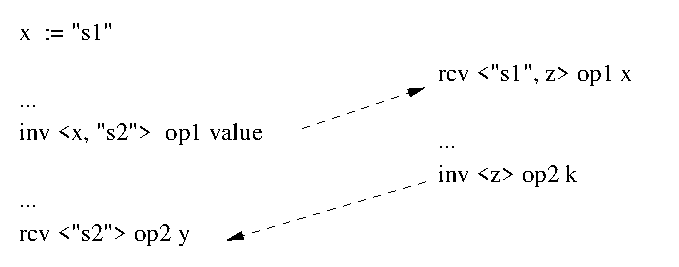
\includegraphics{linguaggio/dia/com}
   \caption[Comunicazione asincrona con Blite]{
   	\textsf{{\small Realizzazione della comunicazione asincrona
   	richiesta-risposta con i construtti della sintassi di Blite}} }
  \label{fig:lin:com}
\end{center}
\end{figure}

La composizione distribuita di diversi processi viene definita dalla categoria
sintattica \emph{Deployments}. Un termine $\xd_1 \xspar \xd_2$ rappresenta la
contemporanea escuzione di tutte le istanze ottenute dalle
definizioni presenti in $\xd_1$ e in $\xd_2$. Un \emph{Deployment}
$\xeng{\xI}{\xcorr}$ è formato dalla definizione di processo $\xI$ con tutte le 
istanze locali a cui è stato associato il \emph{Correlation Set} $\xcorr$. Tale
insieme individua fra tutte le variabili presenti nella definizione del
processo quelle che dovranno essere considerate per valutare la correlazione di un messaggio
ad una particolare istanza. Vedremo come la semantica di Blite definisca tale
processo di attribuzione di un messaggio a una istanza e come tale
semantica sia stata implemetata del nostro engine di esecuzione.
 
In generale si impone la restrizione che un insieme di deployments sia
\emph{ben formato}, nel senso che i nomi nei partner link utilizzati per le
ricezioni non siano condivisi fra diversi deployment. In questo modo ogni
definizione di processo avrà i propri nomi di servizo univoci e dato un nome
sarà sempre possibile individuare un deployment specifico.

In seguito, nella definizione della semantica, si farà uso della notazione
$\bar{\cdot}$, per denotare tuple di valori o variabili, $\bar{\xx}$ può
essere considerata l'abbreviazione di $\arr{\xx_1,
\ldots, \xx_h}$ (con $h \geq 0$). L'ulteriore notazione $\tilde{\cdot}$
indicherà tuple speciali di uno o al massimo due elementi ($\tilde{\xp}$ starà
per $\arr{\xp_1, \xp_2}$ o $\arr{\xp_1}$). Inoltre l'operatore
$\xapp{\xdot}{\xdot}$ permetterà di ottenere la tupla $\arr{\xp,
\xu,\xx_1,\ldots,\xx_h}$ come concatenazione di $\arr{\xp, \xu}$ e
$\arr{\xx_1,\ldots,\xx_h}$ scrivendo $\xapp{\arr{\xp,
\xu}}{\arr{\xx_1,\ldots,\xx_h}}$.
\\

Per concludere si osservi come la sintassi esposta debba ancora essere 
considerata ``astratta'', in quanto non definisce tutti gli aspetti necessari
all'imlemetazione. In particolar modo non definisce i tipi dei valori
attribuibili alle variabili, né la sintassi delle espressioni supportate, e
nemmeno esplicita la precedenza degli operatori di sequenzializzazione,
parallelismo e scelta esterna\footnote{In merito alla precedenza degli
operatori, il documento originale in cui è descritto Blite, afferma che
l'operatore di sequenza $\cdot ; \cdot$ ha precedenza
sull'operatore di parallelismo $\cdot | \cdot$, e che quest'ultimo ha precedenza
sull'operatore di scelta $\cdot + \cdot$}. Di fatto l'implemetazione da noi
realizzata fa riferimento ad una sintassi concreta che definisce in maniera
formale anche questi aspetti. In particolare vedremo come  i semplici
operatori binari siano trasformati in costrutti con 
delimitatori di blocco. In questo modo risulta più semplice
l'implementazione del parser 
%in quanto evita la necessità di eseguire \emph{lookahead}, 
e anche la
precedenza di un attività rispetto l'altra risulta esplicitata nella codifica
stessa dei blocchi. Così il codice risulta più leggibile e più simile nella
struttura sia ai tradizionali linguaggi di programmazione che ad un linguaggio come BPEL basato su XML .
\\

Presentiamo ora la semantica formale in termini operazionali. Le relazioni
semantiche sono definite su termini che includono ulteriori
simboli e costrutti, rispetto a quelli definiti dalla sintassi di Tabella
\ref{tab:syntaxwsbpel}, allo scopo di rappresentare alcuni aspetti dinamici
dell'esecuzione. In particolare vengono introdotti:

\begin{itemize}
  \item \emph{Protected activity}, $\xprot{\xs}$, utilizzato per sostituire
  contesti falliti con i rispettivi compesation handler da eseguire in maniera
  protetta. La sematica chiarirà il significato di esecuzione protetta.
  
  \item \emph{Unsuccessful termination}, $\xstop$, utilizzato per uniformare il
  comportamento delle attività $\xexit$ e $\xthr$.
  
  \item \emph{Message} $\xmsg{\tilde{\xp}}{\xo}{\bar{\xv}}$, utilizzato per
  rappresentare i messaggi prodotti dalle attività invoke.
    
  \item \emph{Scope} dalla forma $\xscope{\xs'}{\xs_f}{\xs_c}{\xs_d}$,
  utilizzato per rappresentare l'evoluzione del contesto
  $\xscopefc{\xs}{\xs_f}{\xs_c}$, in cui il completamento di sottocontesti
  definiti in $\xs$ hanno prodotto l'istallazione di compensation handler
  reppresentati con $\xs_d$.
\end{itemize}

Inotre si introduce il concetto di attività \emph{short-lived} con l'intento
d'individuare un sott'insieme fra tutti i tipi di attività presenti nel
linguaggio. Vedremo che la semantica attribuirà a tali attività la proprietà di
essere immuni alla terminazione (in un certo senso queste attività
dovranno essere considerate atomiche rispetto al processo di terminazione).
Tale insieme è costituito dalla seguenti attività

$$
\textrm{Attività \emph{short-lived}} : \{ \xskip, \xexit,
\xthr, \xstop, \xmsg{\tilde{\xp}}{\xo}{\bar{\xv}} \}
$$

e di seguito una generica attività short-lived sarà indicata con
il simbolo $\xsla$.
\\

La semantica dei termini Blite è definita tramite una congruenza strutturale, e
tramite due relazioni di transizione, una che descrive l'evoluzione delle
istanze in termini di operazioni interne, e una che descrive l'evoluzione del sistema
di deployment attraverso le comunicazioni. 

La \emph{Congruenza Strutturale}, identifica come equivalenti termini
sitatticamente diversi ma che intuitivamente rappresentano il medesimo
comportamento. Essa è definita come la più grande congruenza indotta dalle
equazioni reppresentate in Tabella \ref{tab:congwsbpel}, dove peraltro non sono
riportate le leggi che esplicitano le ovvie proprietà di
commutatività e associatività per gli operatori binari.

%%%%% STRUCTURAL CONG Blite %%%%%
\begin{table}[t]
\begin{small}
$$
\delimite{
\begin{array}{c}
\xs \xpar \xskip \xequiv \xs
\qquad
\xskip\xsucc\xs \xequiv \xs\xsucc\xskip \xequiv \xs
\qquad
\xstop \xpar \xstop \xequiv \xstop
\qquad
\xstop \xsucc \xs \xequiv \xstop
\\[0.2cm]
\xprot{\xprot{\xs}} \xequiv \xprot{\xs}
\qquad
\xprot{\xsla} \xequiv \xsla
\qquad
\xprot{\xmsg{\tilde{\xp}}{\xo}{\bar{\xv}}\, \spar \xs} \xequiv \,
\xmsg{\tilde{\xp}}{\xo}{\bar{\xv}} \, \spar \xprot{\xs}
\\[0.2cm]
\xscopefc{\xs}{\xs_f}{\xs_c} \xequiv
\xscope{\xs}{\xs_f}{\xs_c}{\xskip}
\qquad
(\xmsg{\tilde{\xp}}{\xo}{\bar{\xv}}\, \spar \xs_1)\xsucc\xs_2
\xequiv \, \xmsg{\tilde{\xp}}{\xo}{\bar{\xv}}\, \spar
(\xs_1\xsucc\xs_2)
\\[0.2cm]
\xscope{\xmsg{\tilde{\xp}}{\xo}{\bar{\xv}} \, \spar
\xs}{\xs_f}{\xs_c}{\xs_d} \xequiv\,
\xmsg{\tilde{\xp}}{\xo}{\bar{\xv}}\, \spar
\xscope{\xs}{\xs_f}{\xs_c}{\xs_d} \quad \textrm{if}\ \neg
\nothr{\xs}
\\[0.2cm]
\prooftree \xs \xequiv \xs' \quad \xs_f \xequiv \xs_f' \quad \xs_c
\xequiv \xs_c' \quad \xs_d \xequiv \xs_d' \justifies \
\xscope{\xs}{\xs_f}{\xs_c}{\xs_d} \xequiv\,
\xscope{\xs'}{\xs_f'}{\xs_c'}{\xs_d'}
\endprooftree
\\[0.45cm]
\hline\\[-0.2cm]
\prooftree \xsa \xequiv \xsa' \qquad \xh_f \xequiv \xh_f' \justifies
\ \xeng{\xproc{\xsa}{\xh_f}\xmid\xI}{\xcorr} \xequiv
\xeng{\xI\xmid\xproc{\xsa'}{\xh_f'}}{\xcorr}
\endprooftree
\qquad
\prooftree \xs \xequiv \xs' \justifies \
\xeng{\xinst{\xsigma}{\xs}\xmid\xI}{\xcorr} \xequiv
\xeng{\xI\xmid\xinst{\xsigma}{\xs'}}{\xcorr}
\endprooftree
\\[0.6cm]
\xd_1 \xspar \xd_2 \xequiv \xd_2 \xspar \xd_1
\qquad
(\xd_1 \xspar \xd_2)\, \xspar \xd_3 \xequiv \xd_1 \xspar (\xd_2
\xspar \xd_3)
\qquad
\xeng{\xinst{\xsigma}{\xskip}\xmid\xI}{\xcorr} \xequiv
\xeng{\xI}{\xcorr}
\\[0.2cm]
\xeng{\xinst{\xsigma}{\xstop}\xmid\xI}{\xcorr} \xequiv
\xeng{\xI}{\xcorr}
\qquad
\xeng{\xinst{\xsigma}{\xskip}}{\xcorr} \xspar \xd \xequiv \xd
\qquad
\xeng{\xinst{\xsigma}{\xstop}}{\xcorr} \xspar \xd \xequiv \xd
\end{array}
}
$$
\end{small}
  \vspace*{-1.20cm}
  \caption{Congruenza Strutturale per le attività e i deployment}
  \vspace*{-0.3cm}
  \label{tab:congwsbpel}
\end{table}
%%%%%%%%%%%%%%%%% STRUCTURAL CONG %%%%%%%%%%%%%%%

Dalla congruenza strutturale deduciamo che: l'attività $\xskip$ agisce come
l'elemento identità sia per l'operatore di sequenza che per l'operatore di
parallelismo. La composizione parallela di più attività $\xstop$ è equivalente ad
un'unica $\xstop$, mentre la stessa $\xstop$ premessa nella sequenzializzazione
disabilita le attività successive. L'operatore di protezione $\xprot{\cdot}$
risulta idempotente e le attività short-lived sono da considerarsi implicitamente
protette, in questo modo è espressa la loro immunità alla terminazione. I
messaggi possono essere estratti dall'operatore di protezione.
All'inizio dell'esecuzione di uno scope il compensation handler istallato è da
considerarsi uguale all'attività $\xskip$. Importante è notare come la
produzione di messaggi non blocchi le attività successive, né il completamento
di scope a meno che nello scope stesso non sia attivato un $\xthr$
(quest'ultima possibilità è verificata tramite il predicato $\nothr{\xdot}$ che
verrà formalizzato più avanti). Quest'ultime equazioni concorrono alla
definizione di un modello di comunicazione puramente ascincrono per i processi
Blite. Le equazioni rimanenti risultano particolarmente ovvie, in quanto
estendono la congruenza strutturale all'applicazione dei costrutti di scope,
deployment e composizione di deployment. Per concludere si osservi che istanze
del tipo $\xinst{\xsigma}{\xskip}$ e $\xinst{\xsigma}{\xstop}$ risultano
terminate e possono essere eliminate, equivalentemente deployment contenenti
solamente istanze terminate sono da considerarsi terminate e possono a loro
volta essere eliminate.
\\

\begin{table}[t!]
\begin{small}
$$
\delimite{
\begin{array}{@{\hspace{-.1cm}}l@{\hspace{.3cm}}r@{\hspace{-.1cm}}}
\xinst{\xsigma}{\xinv{\plinv}{\xo}{\bar{\xx}}} \bpeltsarrow{\xtau}
\xinstnostate{\xsigma}{\,\xmsg{\xsigma(\plinv)}{\xo}{\xsigma(\bar{\xx})}}
\ \; \rulelabel{$\x{inv}$}
&
\xinstnostate{\xsigma}{\xrec{\plrec}{\xo}{\bar{\xx}}}
\bpeltsarrow{\xrecl{\plrec\,}{\,\xo\,}{\,\bar{\xx}}}
\xinstnostate{\xsigma}{\xskip} \; \; \rulelabel{$\x{rec}$}
\\
[0.2cm] \xinst{\xsigma}{\xass{\xx}{\xe}}
\bpeltsarrow{\xassl{\xx}{\xsigma(\xe)}}
\xinstnostate{\xsigma}{\xskip} \ \; \rulelabel{$\x{asg}$}
&
\xinstnostate{\xsigma}{\xthr}
\bpeltsarrow{\xthrl}
\xinstnostate{\xsigma}{\xstop}
\ \; \rulelabel{$\x{thr}$}
\\
[0.2cm] \multicolumn{2}{c}{
\xinstnostate{\xsigma}{\xexit}
\bpeltsarrow{\xexitl} \xinstnostate{\xsigma}{\xstop} \ \;
\rulelabel{$\x{term}$}
\qquad\
\xinstnostate{\xsigma}{\xmsg{\tilde{\xp}}{\xo}{\bar{\xv}}}\,
\bpeltsarrow{\xmsgl{\tilde{\xp}\,}{\,\xo\,}{\,\bar{\xv}}}
\xinstnostate{\xsigma}{\xskip} \ \; \rulelabel{$\x{msg}$}
\qquad\
\prooftree \xinst{\xsigma}{\xs} \bpeltsarrow{\xalpha}
\xinstnostate{\xsigma'}{\xs'} \justifies \
\xinst{\xsigma}{\xprot{\xs}} \bpeltsarrow{\xalpha}
\xinstnostate{\xsigma'}{\xprot{\xs'}} \using \;
\rulelabel{$\x{prot}$}
\endprooftree
}
\\[0.2cm]
\multicolumn{2}{c}{
\prooftree \xinst{\xsigma}{\xs_1}
\bpeltsarrow{\xalpha} \xinstnostate{\xsigma'}{\xs_1'} \justifies \
\xinst{\xsigma}{\xs_1\xsucc\xs_2} \bpeltsarrow{\xalpha}
\xinstnostate{\xsigma'}{\xs_1'\xsucc\xs_2} \using \;
\rulelabel{$\x{seq}$}
\endprooftree
\qquad\qquad\quad\
\xinstnostate{\xsigma}{$ $ \sum_{j\in
J}\xrec{\plrec_j}{\xo_j}{\bar{\xx}_j}\recsep\xs_j $ $}
\bpeltsarrow{\xrecl{\plrec_h\,}{\,\xo_h\,}{\,\bar{\xx}_h}}
\xinstnostate{\xsigma}{\xs_h} \ \ \ (h \in J) \ \
\rulelabel{$\xsuml$} }
\\[0.6cm]
%\prooftree
%\xs = \left\{\begin{array}{l@{\hspace{2ex}}l}
%\xs_1 & \textrm{if}\ \xsigma(\xx) = \xtrue\\
%\xs_2 & \textrm{if}\ \xsigma(\xx) = \xfalse\\
%\end{array}\right.
%\justifies \
%\xinst{\xsigma}{\xif{\xx}{\xs_1}{\xs_2}}
%\bpeltsarrow{\xtau}
%\xinstnostate{\xsigma}{\xs}
%\using \; \rulelabel{$\x{if}$}
%\endprooftree
\prooftree \xs = \left\{\begin{array}{l@{\hspace{2ex}}l}
\\[-.60cm]
\xs_1 & \textrm{if}\ \xsigma(\xe) = \xtrue\\[-.15cm]
\xs_2 & \textrm{if}\ \xsigma(\xe) = \xfalse\\
\end{array}\right.
\justifies \
\xinst{\xsigma}{\xif{\xe}{\xs_1}{\xs_2}}
\bpeltsarrow{\xtau}
\xinstnostate{\xsigma}{\xs}
\using \; \rulelabel{$\x{if}$}
\endprooftree
&
%\prooftree \xs' = \left\{\begin{array}{l@{\hspace{2ex}}l}
%\xs\xsucc\xwhile{\xx}{\xs} &
%\textrm{if}\ \xsigma(\xx) = \xtrue\\
%\xskip & \textrm{if}\ \xsigma(\xx) = \xfalse\\
%\end{array}\right.
%\justifies \
%\xinst{\xsigma}{\xwhile{\xx}{\xs}}
%\bpeltsarrow{\xtau}
%\xinstnostate{\xsigma}{\xs'}
%\using \; \rulelabel{$\x{while}$}
%\endprooftree
\prooftree \xs' = \left\{\begin{array}{l@{\hspace{2ex}}l}
\\[-.60cm]
\xs\xsucc\xwhile{\xe}{\xs} &
\textrm{if}\ \xsigma(\xe) = \xtrue\\[-.15cm]
\xskip & \textrm{if}\ \xsigma(\xe) = \xfalse\\
\end{array}\right.
\justifies \
\xinst{\xsigma}{\xwhile{\xe}{\xs}}
\bpeltsarrow{\xtau}
\xinstnostate{\xsigma}{\xs'}
\using \; \rulelabel{$\x{while}$}
\endprooftree
\\[0.80cm]
\multicolumn{2}{c}{
\prooftree
\xinst{\xsigma}{\xs_1}
\bpeltsarrow{\xalpha}
\xinstnostate{\xsigma'}{\xs_1'}
\quad
\xalpha \notin \{\xexitl, \xthrl\}
\quad
\neg (\nothr{\xs_2}\! \vee\, \noexit{\xs_2})
\justifies \
\xinst{\xsigma}{\xs_1 \xpar \xs_2}
\bpeltsarrow{\xalpha}
\xinstnostate{\xsigma'}{\xs_1' \xpar \xs_2}
\using \; \rulelabel{$\x{par}_1$}
\endprooftree
\quad\
\prooftree
\xinstnostate{\xsigma}{\xs_1}
\bpeltsarrow{\xalpha}
\xinstnostate{\xsigma}{\xs_1'}
\quad
\xalpha \in \{\xexitl, \xthrl\}
\justifies \
\xinstnostate{\xsigma}{\xs_1 \xpar \xs_2}
\bpeltsarrow{\xalpha}
\xinstnostate{\xsigma}{\xs_1' \xpar \xhalt{\xs_2}}
\using \; \rulelabel{$\x{par}_2$}
\endprooftree
}
\\[0.7cm]
\xinstnostate{\xsigma}{\xscope{\xskip}{\xs_f}{\xs_c}{\xs_d}}
\bpeltsarrow{\xdonel{\xs_c}}
\xinstnostate{\xsigma}{\xskip} \; \; \rulelabel{$\xdl_1$}
&
\xinstnostate{\xsigma}{\xscope{\xstop}{\xs_f}{\xs_c}{\xs_d}}
\bpeltsarrow{\xtau} \xinstnostate{\xsigma}{\xprot{\xs_d\xsucc\xs_f}}
\; \;  \rulelabel{$\xdl_2$}
\\[0.2cm]
\multicolumn{2}{c}{
\prooftree \xinst{\xsigma}{\xs} \bpeltsarrow{\xalpha}
\xinstnostate{\xsigma'}{\xs'} \quad \xalpha \notin \{\xthrl,\xdonel{\xs''}\}
\justifies
\ \xinst{\xsigma}{\xscope{\xs}{\xs_f}{\xs_c}{\xs_d}}
\bpeltsarrow{\xalpha}
\xinstnostate{\xsigma'}{ \xscope{\xs'}{\xs_f}{\xs_c}{\xs_d}}
\using \; \rulelabel{$\x{exec}$}
\endprooftree
}
\\[0.5cm]
\multicolumn{2}{c}{
\prooftree
\xinstnostate{\xsigma}{\xs}
\bpeltsarrow{\xdonel{\xs''}}
\xinstnostate{\xsigma}{\xs'}
\justifies \
\xinstnostate{\xsigma}{\xscope{\xs}{\xs_f}{\xs_c}{\xs_d}}
\bpeltsarrow{\xtau}
\xinstnostate{\xsigma}{\xscope{\xs'}{\xs_f}{\xs_c}{\xs''\xsucc\xs_d}}
\using \; \rulelabel{$\xdl_3$}
\endprooftree
}
\\[0.5cm]
\multicolumn{2}{c}{
\prooftree
\xinstnostate{\xsigma}{\xs} \bpeltsarrow{\xthrl}
\xinstnostate{\xsigma}{\xs'} \justifies \
\xinstnostate{\xsigma}{\xscope{\xs}{\xs_f}{\xs_c}{\xs_d}}
\bpeltsarrow{\xtau}
\xinstnostate{\xsigma}{\xscope{\xs'}{\xs_f}{\xs_c}{\xs_d}} \using \;
\rulelabel{$\x{fault}$}
\endprooftree
}
\end{array}
}
$$
\end{small}
  \vspace*{-1.20cm}
  \caption[Semantica operazionale per le attività]{Semantica operazionale per
  le attività.}
  \label{tab:allSOS}
  \vspace*{-0.3cm}
\end{table}

L'evoluzione delle attività di una istanza di processo è descritta dalla
relazione di transizione etichettata $\bpeltsarrow{\xalpha}$, le cui regole
sono presentate in Tabella \ref{tab:allSOS}, dove le etichette o azioni
$\xalpha$ sono generate dalla seguente grammatica:

$$
\begin{array}
{r@{\hspace*{.3cm}}c@{\hspace*{.3cm}}l}
\xalpha & ::= &
\xtau \sepgr
\xassl{\xx}{\xv} \sepgr
\xinvl{\tilde{\xp}}{\xo}{\bar{\xv}} \sepgr
\xrecl{\plrec}{\xo}{\bar{\xx}} \sepgr
\xexitl \sepgr \xthrl \sepgr \xdonel{\xs}
\end{array}
$$

in cui i nuovi simboli introdotti devono essere interpretati come le seguenti
azioni:

\begin{itemize}
  \item $\xtau$ indica la produzione di un messaggio o operazioni interne come
  la valutazione di test nella scelta condizionata e nella iterazione
  o l'istallazione/attivazione di compesation handler.
  \item $\xassl{\xx}{\xv}$ indica l'assegnamento del valore $\xv$ alla
  variabile $\xx$.
  \item $\xinvl{\tilde{\xp}}{\xo}{\bar{\xv}}$ e
  $\xrecl{\plrec}{\xo}{\bar{\xx}}$  indicano rispettivamente l'esecuzione di
  una invocazione sull'operazione $\xo$, con il partner link valorizzato a
  $\tilde{\xp}$ e parametri attuali $\bar{\xv}$, e la ricezione sull'operazione
  $\xo$, partner link $\plrec$ e parametri formali $\bar{\xx}$.
  \item $\xexitl$ indica la richiesta di una terminazione forzata di una
  istanza di processo.
  \item $\xthrl$ indica la generazione di una eccezione.
  \item $\xdonel{\xs}$ indica il completamento con successo di uno scope
  che potrà essere eventualmente compensato tramite l'attività $\xs$.
\end{itemize}

La relazione $\bpeltsarrow{\xalpha}$ è definita con l'ausilio della funzione di
stato $\xsigma$ che associa un valore ad ogni variabile dell'istanza a cui è
associata (vi è uno stato distinto e unico per ogni istanza di processo, mentre
non vi è il concetto di stato locale associato ai contesti). In particolare
$\xsigma(\xx)$ restituisce il valore della variabile $\xx$ nello stato $\xsigma$
e $\xsigma(\xe)$ restituisce il risultato della valutazione dell'espressione
$\xe$ nello stato $\xsigma$. La funzione stato $\xsigma$ può essere aggiornata
con $\xsigma'$, scrivendo $\xsigma \xupd \xsigma'$, in modo da avere 

$$
\xsigma \xupd \xsigma'(\xx) = \left\{ 
\begin{array}{ll}
\xsigma'(\xx) & \textrm{se $\xx \in \xdom{\xsigma'}$}\\
\xsigma(\xx) & \textrm{altrimenti}\\
\end{array}
\right.
$$

Bisogna osservare che in alcune regole di Tabella \ref{tab:allSOS} tale
funzione non è esplicitata, per esempio per semplicità si è scritto
$\xinstnostate{\xsigma}{\xs}
\bpeltsarrow{\xalpha} \xinstnostate{\xsigma}{\xs'}$ invece di $\xinst{\xsigma}{\xs} \bpeltsarrow{\xalpha}
\xinstnostate{\xsigma}{\xs'}$.

Alcune funzioni e predicati ausiliari, come già precedentemente osservato, sono
stati introdotti a supporto della definizione semantica. In particolare i
predicati $\noexit{\xs}$ and $\nothr{\xs}$ valutano la capacità di 
$\xs$ di eseguire $\xexit$ o $\xthr$, rispettivamente. Essi sono definiti per
induzione sulla struttura sintattica delle attività e di fatto valgono sempre
falso tranne che per i casi seguenti in cui si ha:

$$
\begin{array}{c}
\noexit{\xexit}
\quad\ \
\nothr{\xthr}
\quad\ \
\prooftree
\noexit{\xs_1}
\justifies \
\noexit{\xs_1 \xsucc \xs_2}
\endprooftree
\qquad
\prooftree
\nothr{\xs_1}
\justifies \
\nothr{\xs_1 \xsucc \xs_2}
\endprooftree

\\[0.7cm]
\prooftree
\noexit{\xs}
\justifies \
\noexit{\xscope{\xs}{\xs_f}{\xs_c}{\xs_d}}
\endprooftree

\qquad

\prooftree
\noexit{\xs}
\justifies \
\noexit{\xprot{\xs}}
\endprooftree

\qquad

\prooftree
\noexit{\xs}
\justifies \
\nothr{\xprot{\xs}}
\endprooftree

\\[0.7cm]
\prooftree
\noexit{\xs_1} \, \vee \, \noexit{\xs_2}  
\justifies \
\noexit{\xs_1 \xpar \xs_2}
\endprooftree

\qquad

\prooftree
\nothr{\xs_1} \, \vee \, \nothr{\xs_2}  
\justifies \
\nothr{\xs_1 \xpar \xs_2}
\endprooftree

\\[0.5cm]
\end{array}
$$

Per rappresentare la semantica della terminazione viene introdotta la
funzione $\xhalt{\xdot}$, che applicata ad un'attività, la restituisce
in modo da lasciare solamente le attività short-lived e quelle protette. Anche
tale funzione è definita sulla struttura sintattica delle attività e si ha che 
$\forall \xs \; \xhalt{\xs} = \xstop$ tranne i seguenti casi
 
$$
\begin{array}{c}
\xhalt{\xsla}=\xsla
\qquad \quad \
\xhalt{\xprot{\xs}}=\xprot{\xs}
\qquad \quad \
\xhalt{\xs_1\xsucc\xs_2}  = \xhalt{\xs_1}
\\[0.2cm]
\xhalt{\xscope{\xs}{\xs_f}{\xs_c}{\xs_d}} = \xscope{\xhalt{\xs}}{\xs_f}{\xs_c}{\xs_d}
\quad
\xhalt{ \xs' \xpar \xs'' } =  \xhalt{\xs'} \xpar \xhalt{\xs''}  
\end{array}
$$
in cui $\xs_1$ non può essere congruente a $\xskip$ o a
$\xmsg{\tilde{\xp}}{\xo}{\bar{\xv}}$, o alla composizione parallela
di essi.
\\

Commentiamo ora le regole di Tabella \ref{tab:allSOS}.
\begin{description}
  \item[\rulelabel{$\x{inv}$} \rulelabel{$\x{asg}$}] 
  Affermano che le attività di invocazione e di assegnamento
  possono procedere solamente se i loro argomenti sono espressioni
  chiuse (cioè senza varibili non inizializzate). Inoltre \rulelabel{$\x{inv}$} insieme 
  alla successiva \rulelabel{$\x{msg}$} e alla congruenza strutturale
  definisce la semantica asincrona per la comunicazione. Si osservi infatti il
  seguente comportamento:
  $$
  \begin{array}{c}
  	\xinv{\plinv}{\xo}{\bar{\xx}} \xsucc \xs 
  	\; \bpeltsarrow{\xtau} \;
  	\xinstnostate{\xsigma}{\,\xmsg{\xsigma(\plinv)}{\xo}{\xsigma(\bar{\xx})}} \xsucc \xs 
  	\; \xequiv \; 
  	( \xmsg{\xsigma(\plinv)}{\xo}{\xsigma(\bar{\xx})} \xpar \xskip) \xsucc \xs
  	\\ \xequiv \;
  	\xmsg{\xsigma(\plinv)}{\xo}{\xsigma(\bar{\xx})} \xpar (\xskip \xsucc \xs )
  	\; \xequiv \;
  	\xmsg{\xsigma(\plinv)}{\xo}{\xsigma(\bar{\xx})} \xpar \xs 
  \end{array}
  $$
   
  \item[\rulelabel{$\x{rec}$}] Un'operazione di ricezione offre la
  possibilità di invocazione di un'operazione locale su un fissato partner
  link. Da osservare che a differenza della invocazione la ricezione blocca le
  attività sequenzialmente successive.
  
  \item[\rulelabel{$\x{thr}$} \rulelabel{$\x{term}$}] Rappresentono
  rispettivamente la produzione di un'eccezione e di una richiesta di
  terminazione per l'istanza corrente.
  
  \item[\rulelabel{$\x{msg}$}] Un messaggio può essere consumato
  indipendentemente dalla sua generazione.
  
  \item[\rulelabel{$\x{prot}$}] Il costrutto $\xprot{\xs}$ permette la
  normale esecuzione di $\xs$ al suo interno. Poiché
  $\xhalt{\xprot{\xs}}=\xprot{\xs}$, con l'operatore $\xprot{\cdot}$ si ottiene
  la protezione di $\xs$ dalle richieste esterne di terminazione.
 
  \item[\rulelabel{$\x{seq}$} \rulelabel{$\x{pick}$} \rulelabel{$\x{if}$}
  \rulelabel{$\x{while}$}] Esprimono una semantica standard rispetto ai
  tradizionali linguaggi di programmazione e alle più comuni algebre di
  processo che prevedono l'operatore di scelta esterna.
  
  
  \item[\rulelabel{$\x{par}_1$} \rulelabel{$\x{par}_2$}] Esprimono la semantica
  caratteristica di BPEL riguardo alla terminazione nella composizione
  parallela con attività fallite. Di fatto esse affermano che l'esecuzione di
  attività parallele evolve come atteso se nessuna di esse ha sollevato
  un'eccezione o richiesto una terminazione. Viceversa, se questo accade, tutti
  i rami della composizione parallela vengono terminati. Si ricordi anche che 
  per definizione $\xhalt{ \xs' \xpar \xs'' } =  \xhalt{\xs'} \xpar
  \xhalt{\xs''}$.
  
  \item[\rulelabel{$\xdl_1$} \rulelabel{$\xdl_3$}] Esprimono la caratteristica
  di BPEL secondo cui contesti completati con successo istallano nei rispettivi
  contesti padre i loro compensation handler per un'eventuale successiva
  compensazione. Il contesto padre colleziona in sequenza i compensation halder
  di contesti figli completati \rulelabel{$\xdl_3$}. Questa
  semantica, differentemente dalla specifica informale di BPEL, prevede che i
  compesation handler siano mantenuti attraverso un solo grado di parentela
  nella gerarchia dei contesti. Difatti un contesto completato istalla nel suo
  padre solo il suo conpensation handler e non quelli istallati dai suoi figli.
  Una semantica alternativa poteva essere:
  $$
  \xinstnostate{\xsigma}{\xscope{\xskip}{\xs_f}{\xs_c}{\xs_d}}
\bpeltsarrow{\xdonel{\xs_d;\xs_c}}
\xinstnostate{\xsigma}{\xskip} 
  $$
  in cui si mantengono anche i conpensation handler precedentemente istallati.

  \item[\rulelabel{$\x{exec}$}] Se non si producono eccezioni l'esecuzione
  interna ad uno scope procede come atteso. Da osservare che questa regola è da
  applicare anche nel caso in cui $\xs$ richieda una terminazione 
  (${\xs} \bpeltsarrow{\xexitl} \xs' \bpeltsarrow{} \ldots {\xstop}$); qui a
  differenza di \rulelabel{$\x{fault}$} l'azione $\xexitl$ viene propagata
  anche al di fuori del contesto per produrre la terminazione di tutta
  l'istanza e successivamente tramite l'applicazione di \rulelabel{$\xdl_2$} vengono eseguiti i
  compesation handler istallati e il fault hadler del contesto corrente.
  
  \item[\rulelabel{$\xdl_2$}] In uno scope in cui la contest activity giunge a 
  $\xstop$ a causa di una eccezione o di una richiesta di terminazione,
  attraverso una transizione interna si attiva l'esecuzione protetta dei
  compensation handler istallati e del fault handler. Importante è osservare
  come l'esecuzione dell'ambiente protetto avvenga nello stato attuale
  dell'istanza.
  
  \item[\rulelabel{$\x{fault}$}] La sollevazione di un'eccezione in $\xs$ non
  viene propagata al di fuori dello scope, ma gestita tramite una transizione
  interna.  La successiva evoluzione di ${\xs} \bpeltsarrow{\xthrl} \xs'
  \bpeltsarrow{} \ldots \, {\xstop}$ in cui vengono terminati gli eventuali
  rami paralleli, porterà all'applicazione di \rulelabel{$\xdl_2$}. 
\end{description}

Abbiamo definito il comportamento delle attività interne delle istanze di
processo, vediamo ora come avviene la creazione di tali istanze e la
comunicazione in sistemi composti da più deployment. Il comportamento di
questi ultimi è definito dalla relazione di riduzione $\bpelredarrow{}$,
le cui regole sono presentate in Tabella \ref{tab:deploySOS}.

%%%%%%%%%%%%%%%%%%%%%%%%%%%%%%%%%%%%%%%%%%%%%%%%%%%%%%%%%%%%%%%%%%%%%%%%%%%%%%%%
% RIDUZIONE PER I deployment
\begin{table}[t]
\begin{small}
$$
\delimite{
\begin{array}{c}
\prooftree
\xinstnostate{\xsigma_1}{\xs_1} \bpeltsarrow{\ialpha_1}
\xinstnostate{\xsigma_1}{\xs_1'} \quad
\xinstnostate{\xsigma_2}{\xs_2} \bpeltsarrow{\oalpha_2}
\xinstnostate{\xsigma_2}{\xs_2'}
\quad \xxnewmatch{\xcorr_1}{\xsigma_1}{\talpha_1}{\talpha_2} =
\xsigma_1' \quad \neg\,
(\,\xnoCONF{\xcorr_1}{\xinst{\xsigma_1}{\xs_1} \xmid \xI_1}
{\talpha_2}{\length{\,\xsigma_1'}}\!)
\justifies \ \xeng{\xinst{\xsigma_1}{\xs_1}\xmid\xI_1}{\xcorr_1}
\xspar \xeng{\xinst{\xsigma_2}{\xs_2}\xmid\xI_2}{\xcorr_2}
\bpelredarrow{} \xeng{\xinst{\xsigma_1 \xupd
\xsigma_1'}{\xs_1'}\xmid\xI_1}{\xcorr_1} \xspar
\xeng{\xinst{\xsigma_2}{\xs'_2}\xmid\xI_2}{\xcorr_2} \using \;
\rulelabel{$\x{com}$}
\endprooftree
\\
\\
\prooftree
\xinstnostate{\emptyset}{\xscopefc{\xsa}{\xh_f}{\xskip}}
\bpeltsarrow{\ialpha_1} \xinstnostate{\emptyset}{\xs_1} \quad
\xinstnostate{\xsigma_2}{\xs_2} \bpeltsarrow{\oalpha_2}
\xinstnostate{\xsigma_2}{\xs_2'} \quad
\xxnewmatch{\xcorr_1}{\emptyset}{\talpha_1}{\talpha_2} = \xsigma_1
\!\! \quad \neg\,
(\xnoCONF{\xcorr_1}{\xI_1}{\talpha_2}{\length{\,\xsigma_1}}\!)
\justifies \ \xeng{\xproc{\xsa}{\xh_f} \xmid \xI_1}{\xcorr_1} \xspar
\xeng{\xinst{\xsigma_2}{\xs_2} \xmid  \xI_2}{\xcorr_2}
\bpelredarrow{} \xeng{\xinst{\xsigma_1}{\xs_1} \xmid
\xproc{\xsa}{\xh_f} \xmid \xI_1}{\xcorr_1} \xspar
\xeng{\xinst{\xsigma_2}{\xs_2'} \xmid \xI_2}{\xcorr_2} \using \;
\rulelabel{$\x{new}$}
\endprooftree
\\
\\
\prooftree \xinst{\xsigma}{\xs} \bpeltsarrow{\xassl{\xx}{\xv}}
\xinstnostate{\xsigma}{\xs'} \quad
\xxnewmatch{\xcorr}{\xsigma}{\xx}{\xv} = \xsigma' \justifies \
\xeng{\xinst{\xsigma}{\xs} \xmid \xI}{\xcorr} \bpelredarrow{}
\xeng{\xinst{\xsigma \xupd \xsigma'}{\xs'} \xmid \xI}{\xcorr} \using
\; \rulelabel{$\x{var}$}
\endprooftree
\qquad\qquad
\prooftree \xd_1 \bpelredarrow{} \xd_1' \justifies \ \xd_1 \xspar
\xd_2 \bpelredarrow{} \xd_1' \xspar \xd_2 \using \;
\rulelabel{$\x{part}$}
\endprooftree
\\
\\
\prooftree \xinst{\xsigma}{\xs} \bpeltsarrow{\xalpha}
\xinstnostate{\xsigma'}{\xs'} \quad \xalpha \notin\{
\ialpha_1,\, \oalpha_2,\, \xassl{\xx}{\xv} \} \justifies \
\xeng{\xinst{\xsigma}{\xs} \xmid \xI}{\xcorr} \bpelredarrow{}
\xeng{\xinst{\xsigma}{\xs'} \xmid \xI}{\xcorr} \using \;
\rulelabel{$\x{enab}$}
\endprooftree
\qquad\qquad
\prooftree \xd \xequiv \xd_1 \quad \xd_1 \bpelredarrow{} \xd_2 \quad
\xd_2 \xequiv \xd' \justifies \ \xd \bpelredarrow{} \xd' \using \;
\rulelabel{$\x{cong}$}
\endprooftree
\end{array}
}
$$
\end{small}
  \vspace*{-1.20cm}
  \caption[Regole di riduzione per deployment]{Regole di riduzione per i
  deployment (si consideri $\talpha_1 = \xapp{\plrec}{\xapp{\xo}{\bar{\xx}}}$ e 
  \mbox{$\talpha_2 =
  \xapp{\tilde{\xp}}{\xapp{\xo}{\bar{\xv}}}$}).}
  \label{tab:deploySOS}
  \vspace*{-0.3cm}
\end{table}
%%%%%%%%%%%%%%%%%%%%%%%%%%%%%%%%%%%%%%%%%%%%%%%%%%%%%%%%%%%%%%%%%%%%%%%%%%%%%%%%

La problematica fondamentale è quella di individuare fra le varie istanze di un
deployment quella predisposta alla ricezione di un messaggio, o capire se il
sopraggiungere di un messaggio debba causare la creazione di una nuova istanza.

Nella definizione originale di Blite è stato scelto un approccio puramente
semantico, nel senso che né la sitassi né la struttura dei messaggi prevedono la
presenza di informazioni aggiuntive che possono essere utilizzate per guidare
tali scelte.

Di fatto si è scelto di definire un ordinamento fra tutte le istanze di
processo che concorrono alla ricezione di un determinato messaggio e di dare la
possibilità di consumare il messaggio solo alle prime istanze dell'ordinamento.
Talvolta tale ordinamento può individuare più di un'istanza destinataria
del messaggio, in questo caso la semantica non specifica ulteriormente la scelta
e consente un comportamento non deterministico.

In maniera informale l'ordinamento si basa sul seguente criterio: ``i messaggi
che giungono alle porte di una definizione di processo possono, tramite i
parametri formali, aggiungere più o meno informazione nello stato di una istanza
che riceve. Un messaggio costituito dalla tupla $\arr{\xv_1, \ldots, \xv_n}$,
tramite i parametri formali $\arr{\xx_1, \ldots, \xx_n}$ ha \emph{grado di
definizione} $k \; (k \le n)$, se il messaggio definisce o ridefinisce con nuovi
valori esattamente $k$ variabili formali e lascia immutato lo stato delle
restanti $n - k$. Un messaggio può essere consumato solamente da una fra le
instanze con grado di definizione minimo''. Insieme a questa regola si impone il
vincolo generale che l'assegnamento ad una variabile inclusa nel correlation set
può essere fatto una sola volta, cioè non è possibile assegnare un valore
diverso ad una variabile del correlation set già precedetemente inizializzata.
Se ne conclude che non è possibile leggere un messaggio che assegnarebbe un
valore diverso ad una varibile di correlazione già precedentemente
inizializzata.

Questi ragionamenti vengono formalizzati nella seguente funzione
$\xxnewmatch{\xcorr}{\xsigma}{\bar{\xx}}{\bar{\xv}}$, che prende un correlation
set $\xcorr$, una funzione di stato $\xsigma$, una tupla di variabili $\xx$ e
un tupla di valori $\xv$ e restituisce una funzione di stato eventualmente anche vuota
su un sottoinsieme delle variabili di $\bar{\xx}$:

$$
\begin{array}{c}
\xxnewmatch{\xcorr}{\xsigma}{\xx}{\xv} =
\left\{
\begin{array}{l@{\hspace{2ex}}l}
\\[-.50cm]
\updat{\xx}{\xv} & \textrm{if}\ \xx \notin \xcorr \vee ( \xx \in \xcorr\ \wedge
\xx \notin \xdom{\xsigma})
\\[-.05cm] \emptyset & \textrm{if}\ \xx \in \xcorr
\wedge \updat{\xx}{\xv} \in \xsigma \\
\end{array}
\right.
\\[.7cm]
%\xxnewmatch{\xcorr}{\xsigma}{\xv}{\xv} =
%\emptyset \qquad
\xxnewmatch{\xcorr}{\xsigma}{\arr{}}{\arr{}} =
\emptyset
\\[.7cm]
\prooftree
\xxnewmatch{\xcorr}{\xsigma}{\xx_1}{\xv_1} = \xsigma'
\quad
\xxnewmatch{\xcorr}{\xsigma}{\bar{\xx}_2}{\bar{\xv}_2} = \xsigma''
\justifies \
\xxnewmatch{\xcorr}{\xsigma}{(\xx_1,\bar{\xx}_2)}{(\xv_1,\bar{\xv}_2)} =
\xsigma' \xupd \xsigma''
\endprooftree
\\[.7cm]
\end{array}
$$
\label{pag:match}


Si osservi come $\xxnewmatch{\xcorr}{\xsigma}{\bar{\xx}}{\bar{\xv}}$ non sia
definita nel caso in cui le tuple $\bar{\xx}$ e $\bar{\xv}$ abbiano diversa
lunghezza e quando si abbia per un qualche $i$ che $\xx_i \in \xcorr$ e
$\updat{\xx_i}{\xv'} \in \xsigma$ con $\xv' \neq \xv_i$. 
Quest'ultimo fatto impone quanto precedentemente detto che un'istanza non possa
ricevere messaggi i cui valori assegnati alle variabili attuali non siano
compatibili con lo stato del correlation set.

\begin{table}[t!]
\begin{small}
$$
\delimite{
\begin{array}{c}
% \begin{array}{@{\hspace{-.2cm}}l@{\hspace{.5cm}}l@{\hspace{-.4cm}}}
% \xxnewmatch{\xcorr}{\xsigma}{\xv}{\xv} =
% \emptyset
% &
% \xxnewmatch{\xcorr}{\xsigma}{\xx}{\xv} =
% \left\{
% \begin{array}{l@{\hspace{2ex}}l}
% \\[-.50cm]
% \updat{\xx}{\xv} & \textrm{if}\ \xx \notin \xcorr \vee ( \xx \in \xcorr\ \wedge
% \xx \notin \xdom{\xsigma})
% \\[-.05cm] \emptyset & \textrm{if}\ \xx \in \xcorr
% \wedge \updat{\xx}{\xv} \in \xsigma \\
% \end{array}
% \right.
% \\[.7cm]
% \xxnewmatch{\xcorr}{\xsigma}{\arr{}}{\arr{}} =
% \emptyset
% &
% \prooftree
% \xxnewmatch{\xcorr}{\xsigma}{\xw_1}{\xv_1} = \xsigma'
% \quad
% \xxnewmatch{\xcorr}{\xsigma}{\bar{\xw}_2}{\bar{\xv}_2} = \xsigma''
% \justifies \
% \xxnewmatch{\xcorr}{\xsigma}{(\xw_1,\bar{\xw}_2)}{(\xv_1,\bar{\xv}_2)} =
% \xsigma' \xupd \xsigma''
% \endprooftree
% \end{array}
% \vspace{.3cm}\\
%
%\begin{array}{c}
%\xxnewmatch{\xcorr}{\xsigma}{\xx}{\xv} =
%\left\{
%\begin{array}{l@{\hspace{2ex}}l}
%\updat{\xx}{\xv} & \textrm{if}\ \xx \notin \xcorr \vee ( \xx \in \xcorr\ \wedge \xx \notin \xdom{\xsigma})\\
%\emptyset & \textrm{if}\ \xx \in \xcorr \wedge \updat{\xx}{\xv} \in \xsigma \\
%\end{array}
%\right.
%\\[.5cm]
%\xxnewmatch{\xcorr}{\xsigma}{\xv}{\xv} =
%\emptyset
%\qquad\ \
%\prooftree
%\xxnewmatch{\xcorr}{\xsigma}{\xw_1}{\xv_1} = \xsigma'
%\quad
%\xxnewmatch{\xcorr}{\xsigma}{\bar{\xw}_2}{\bar{\xv}_2} = \xsigma''
%\justifies \
%\xxnewmatch{\xcorr}{\xsigma}{(\xw_1,\bar{\xw}_2)}{(\xv_1,\bar{\xv}_2)} =
%\xsigma' \xupd \xsigma''
%\endprooftree
%\vspace{.3cm}\\
%
%\hline\\
\prooftree
\length{\xxnewmatch{\xcorr}{\xsigma}{\xapp{\plrec}{\xapp{\xo}{\bar{\xx}}}}{\xapp{\tilde{\xp}}{\xapp{\xo}{\bar{\xv}}}}} < \xnum
\justifies \
\xnoCONF{\xcorr}{\xinst{\xsigma}{\xrec{\plrec}{\xo}{\bar{\xx}}\recsep\xs}}{\xapp{\tilde{\xp}\,}{\xapp{\,\xo\,}{\,\bar{\xv}}}}{\xnum}
\endprooftree
\qquad\,\,
\prooftree
\exists\, h \in J \, . \,
\length{\xxnewmatch{\xcorr}{\xsigma}{\xapp{\plrec_h}{\xapp{\xo_h}{\bar{\xx}_h}}}{\xapp{\tilde{\xp}}{\xapp{\xo}{\bar{\xv}}}}} < \xnum
\justifies \
\xnoCONF{\xcorr}{\xinst{\xsigma}{$ $  \sum_{j \in J}\xrec{\plrec_j}{\xo_j}{\bar{\xx}_j}\recsep\xs_j $ $}}{\xapp{\tilde{\xp}\,}{\xapp{\,\xo\,}{\,\bar{\xv}}}}{\xnum}
\endprooftree
\\[0.6cm]
\prooftree
\xnoCONF{\xcorr}{\xinst{\xsigma}{\xs_1}}{\xapp{\tilde{\xp}\,}{\xapp{\,\xo\,}{\,\bar{\xv}}}}{\xnum}
\justifies \
\xnoCONF{\xcorr}{\xinst{\xsigma}{\xs_1\xsucc\xs_2}}{\xapp{\tilde{\xp}\,}{\xapp{\,\xo\,}{\,\bar{\xv}}}}{\xnum}
\endprooftree
\hspace{3cm}
\prooftree
\xnoCONF{\xcorr}{\xinst{\xsigma}{\xs_1}}{\xapp{\tilde{\xp}\,}{\xapp{\,\xo\,}{\,\bar{\xv}}}}{\xnum}
\ \vee\
\xnoCONF{\xcorr}{\xinst{\xsigma}{\xs_2}}{\xapp{\tilde{\xp}\,}{\xapp{\,\xo\,}{\,\bar{\xv}}}}{\xnum}
\justifies \
\xnoCONF{\xcorr}{\xinst{\xsigma}{\xs_1 \xpar \xs_2}}{\xapp{\tilde{\xp}\,}{\xapp{\,\xo\,}{\,\bar{\xv}}}}{\xnum}
\endprooftree
\\[0.6cm]
\prooftree
\xnoCONF{\xcorr}{\xinst{\xsigma}{\xs}}{\xapp{\tilde{\xp}\,}{\xapp{\,\xo\,}{\,\bar{\xv}}}}{\xnum}
\justifies \
\xnoCONF{\xcorr}{\xinst{\xsigma}{\xprot{\xs}}}{\xapp{\tilde{\xp}\,}{\xapp{\,\xo\,}{\,\bar{\xv}}}}{\xnum}
\endprooftree
\qquad \quad\,\,
\prooftree
\xnoCONF{\xcorr}{\xinst{\xsigma}{\xs}}{\xapp{\tilde{\xp}\,}{\xapp{\,\xo\,}{\,\bar{\xv}}}}{\xnum}
\justifies \
\xnoCONF{\xcorr}{\xinst{\xsigma}{\xscope{\xs}{\xs_f}{\xs_c}{\xs_d}}}{\xapp{\tilde{\xp}\,}{\xapp{\,\xo\,}{\,\bar{\xv}}}}{\xnum}
\endprooftree
\qquad \quad\,\,
\prooftree
\xnoCONF{\xcorr}{\xinst{\xsigma}{\xs}}{\xapp{\tilde{\xp}\,}{\xapp{\,\xo\,}{\,\bar{\xv}}}}{\xnum}
\ \vee\
\xnoCONF{\xcorr}{\xI}{\xapp{\tilde{\xp}\,}{\xapp{\,\xo\,}{\,\bar{\xv}}}}{\xnum}
\justifies \
\xnoCONF{\xcorr}{\xinst{\xsigma}{\xs} \xmid \xI}{\xapp{\tilde{\xp}\,}{\xapp{\,\xo\,}{\,\bar{\xv}}}}{\xnum}
\endprooftree
\end{array}
}
$$
\end{small}
  \vspace*{-1.20cm}
  \caption[Definizione predicato match di ricezione]{Definizione del predicato
  $\xnoCONF{\xcorr}{\xI}{\xapp{\tilde{\xp}\,}{\xapp{\,\xo\,}{\,\bar{\xv}}}}{\xnum}$. 
  %C'è un'attività di ricezione attiva sul partner link $\tilde{\xp}$ e
  %operazione $\xo$ che può essere i match con i valori del
  %messaggio $\bar{\xv}$?
  }
  \label{tab:barbeRec}
  \vspace*{-.3cm}
\end{table}

Con la funzione  $\xxnewmatch{\cdot}{\cdot}{\cdot}{\cdot}$ è
possibile definire il predicato
$\xnoCONF{\xcorr}{\xI}{\xapp{\tilde{\xp}\,}{\xapp{\,\xo\,}{\,\bar{\xv}}}}{\xnum}$,
che valuta se un'istanza di processo $\xI$ con correlation set $\xcorr$ ha
un'attività di ricezione attiva che possa ricevere il messaggio
$\xapp{\tilde{\xp}\,}{\xapp{\,\xo\,}{\,\bar{\xv}}}$ con un grado di definizione
minore di $n$. In Tabella \ref{tab:barbeRec} tale predicato viene definito
induttivamente sulla struttura sintattica di $\xI$

A questo punto il comportamento descritto dalle regole di Tabella
\ref{tab:deploySOS} risulta abbastanza intuitivo e può essere sintetizzato nel
seguente modo:

\begin{description}
\item[\rulelabel{$\x{com}$}] Afferma che la comunicazione fra due istanze di
 processo può avvenire solo se si realizza il matching, in rispetto dello stato
 di correlazione, dei valori del messaggio con le variabili di ricezione.
 Ovviamente ci deve essere anche uguaglianza sintattica fra i partner link e
 il nome dell'operazione. Tale regola afferma anche che fra tutte le istanze
 con un'attività di ricezione attiva conforme con i partner link e l'operazione
 del messaggio in arrivo, se ne debba segliere una con grado di
 definizione minimo.
 \item[\rulelabel{$\x{new}$}] Descrive la creazione di una nuova istanza di
 processo a partire dalla definizione $\xproc{\xsa}{\xh_f}$ a seguito
 dell'arrivo di un messaggio $\talpha_2 =
  \xapp{\tilde{\xp}}{\xapp{\xo}{\bar{\xv}}}$ che risulti in matching con una delle start activity della
 definizione stessa. La nuova istanza verrà creata solo se non
 c'è già un'istanza capace di ricevere il messaggio con un grado di
 definizione minore della start activity.
 \item[\rulelabel{$\x{var}$}] Afferma quanto già precedentemente detto che
 l'assegnamento di un valore $\xv$ ad una variabile $\xx$ del correlation set
 su uno stato $\xsigma$ può avvenire solo se $ \xx \notin dom(\xsigma)$ o se $
 \updat{\xx}{\xv} \in \xsigma$.
 \item[\rulelabel{$\x{part}$} \rulelabel{$\x{pass}$} \rulelabel{$\x{cong}$}]
 Tali regole risultano particolarmente ovvie ed esprimono rispettivamente
 l'evoluzione parallela di un sistema di deployment, l'esecuzione
 indipendente delle operazioni interne in ciascuna istanza, l'uguaglianza delle
 riduzioni di deployment strutturalmente congruenti.
\end{description}

%%%%%%%%%%%%%%%%%%%%%%%%%%%%%%%%%%%%%%%%%%%%%%%%%%%%%%%%%%%%%%%%%%%%%%%%%%%%%%%%
% SINTASSI CONCRETA
\section{Una grammatica per un compilatore 
%(??o Parser??)
}
\label{gram}

Il primo passo per lo sviluppo di un motore di esecuzione per Blite è la
realizzazione di un parser per l'analisi di programmi ottenibili dalla sintassi
presentata in Tabella \ref{tab:syntaxwsbpel}. Un parser è il software predisposto
alla realizzazione dell'\emph{Analisi Sintattica}, cioè del procedimento che
riconosce la struttura del programma sorgente e costruisce l'\emph{Albero
Sintattico} (\emph{Abstract Sintatic Tree - AST}) associato. Come già osservato
la sintassi esposta, pur specificando in modo formale i termini del linguaggio,
non si presta ad essere implementata direttamente, in quanto per esempio
presenta regole del tipo 
$$
\begin{array}{rcl}
\xs & ::= & \ldots \quad
\xs \xsucc\xs  \!\sepgr\! \xs \xpar \xs \quad \ldots 
\end{array}
$$
che la rendono ambigua, per cui ad una frase del linguaggio può corrispondere
più di un albero sintattico. Risulta chiaro quindi che il primo obiettivo è
stato quello di ottenere una grammatica direttamente implementabile 
dal cui linguaggio sia possibile ottenere i programmi Blite. Di seguito
chiameremo termini Blite gli elementi del linguaggio derivato dalla sintassi di
Tabella \ref{tab:syntaxwsbpel}, mentre chiameremo programmi Blite le frasi
del linguaggio da noi realmente implementato.
\\

\subsubsection{Cenni di teroria dei linguaggi.}
Dalla teoria sappiamo che le grammatiche per generare linguaggi
analizzabili con parser deterministici, cioè che non fanno uso di tecniche di
backtraking, sono raggruppabili in sotto classi specifiche fra tutte le
possibili grammatiche context free. In particolar modo risultano fondamentali
per la realizzazione di analizzatori sintattici le seguenti classi di
grammatiche:
\begin{itemize}
  \item \textbf{LL(k)}: Per cui risulta possibile realizzare parser top-down
  deterministici che utilizzano al più $k$ simboli non ancora riconosciuti
  della frase di input.
  \item \textbf{LR(k)}: Per cui risulta possibile realizzare parser bottom-up
  deterministici che utilizzano al più $k$ simboli non ancora riconosciuti
  della frase di input.
\end{itemize}

I parser top-down costruiscono l'albero sintattico dalla radice (simbolo
iniziale della grammatica) alle foglie (simboli terminali della frase di
input) secondo la derivazione canonica sinistra, mentre quelli bottom-up
realizzano l'albero sintattico dalle foglie alla radice seguendo la riduzione
destra. 

La derivazione è quel processo che a partire dal simbolo iniziale della
grammatica $S$ arriva alla frase di input applicando ad ogni passo una
sostituzione di un simbolo non terminale $X$ con una parte destra $Y$ presente in
una regola della grammatica del tipo $X ::= Y$. 

Una derivazione può essere scritta come 
$$ S \Rightarrow \cdots \Rightarrow
abcX\ldots \Rightarrow abcY\ldots \cdots \Rightarrow abcdeZ\ldots \Rightarrow
\cdots \Rightarrow abcdef\ldots mn $$ 
in cui l'ultima stringa è formata solo da
terminali. Con il simbolo $ \Rightarrow^*$ si intendono zero o più passi
successivi e con $\Rightarrow^+$ uno o più passi successivi. I singoli passi
della derivazione legano forme di frasi ammesse dalla grammatica, dove una forma
di frase non è altro che una stringa $s \in V^*$, con $V$ insieme dei terminali e
non terminali della grammatica. In un'analisi top-down si realizza la
derivazione canonica sinistra, cioè si impone la sostituzione del simbolo
non terminale che compare più a sinistra nella forma di frase corrente. Quindi
quest'ultima avrà sempre una forma del tipo $aXw$ con $a \in VT^*$ ($VT$ insieme
dei simboli terminali del linguaggio), $X$ simbolo non terminale corrente e $w
\in V^*$. La stringa $a$ costituirà un prefisso della frase di input e
indicherà la parte di essa già riconosciuta. 

Analogamente alla derivazione canonica sinistra si definisce la derivazione
canonica destra che sceglie di sostituire il simbolo non terminale che
compare più a destra nella forma di frase corrente. L'analisi bottom-up realizza
la riduzione destra che è la sequenza inversa della derivazione canonica destra.

In generale con le grammatiche LR si riesce a rappresentare un numero
maggiore di linguaggi rispetto alle grammatiche LL, cioè l'insieme dei
linguaggi generati con grammatiche LL è contenuto nell'insieme dei linguaggi
generati con grammatiche LR; con quest'ultime però risulta molto più complessa
la realizzazione del parser, in quanto è necessario implementare algoritmi e
strutture dati più raffinati.

Inoltre le grammatiche LL hanno caratteristiche che le rendono facilmente
individuabili, e da una generica grammatica, come quella di
Tabella \ref{tab:syntaxwsbpel}, si può ottenere un grammatica LL applicando i seguenti
passi:\footnote{Per una trattazione formale riguardo al riconoscimento di
grammatiche LL(k) si rimanda ai testi specifici della teoria del linguaggi
formali come \cite{Bruno} e \cite{DragonBook}.} 
\begin{itemize}
  \item Eliminazione della ricorsione sinistra diretta o indiretta. Una
  grammatica presenta ricorsione sinistra quando ammette derivazioni del tipo
 $X \Rightarrow^+ Xu$, dove $X \in VN$ e $u \in V^+$ (la ricorsione diretta si
 ha banalmente quando sono presenti regole del tipo $X ::= Xu$), in tal caso
 l'analizzatore top-down può entrare in un ciclo infinito. Esiste un algoritmo
 per eliminare tale problema (si veda \cite{Bruno}), ma in generale può
 essere evitato semplicemente aggiungendo nuovi non terminali e riorganizzando
 le regole. Per esempio la seguente grammatica 
 $$
 \begin{array}{rcl} 
  E & ::= & E + T \; | \; E - T \; |\; T \;|\; -T \\
  T & ::= & T * F \; | \; F \\
  F & ::= & (E) \; | \; i \\
 \end{array}
 $$
 
 che presenta ricorsione sinistra può essere trasformata nella grammatica
 $$
 \begin{array}{rcl} 
  E  & ::= & TE' \; | \; - TE' \\
  E' & ::= & +TE' \; | \; - TE' \; | \; \epsilon \\
  T  & ::= &  FT' \\
  T' & ::= & *FT' \; | \; \epsilon \\
  F & ::= & (E) \; | \; i \\
 \end{array}
 $$
 che ne è priva.
 
  \item Fattorizzazione sinistra. Questo procedimento serve ad eliminare un
  eventuale prefisso comune a due parti destre di regole associate allo stesso
  simbolo non terminale, cosa che in generale porta non determinismo nel
  processo di derivazione canonica sinistra. Se, ad esempio, una regola della grammatica
  è del tipo $A ::= yv \;|\; yw$ con $y \in V^+$, $v
  \in V^*$ e $w \in V^+$ e le stringhe $v$, $w$ non hanno prefissi comuni,
  l'analizzatore top-down, quando espande il simbolo non terminale $A$ non può,
  in generale, scegliere con certezza la parte destra di A da usare,
  guardando un solo simbolo (o anche più di uno ma in numero determinato) in
  avanti nella frase di input. Avrebbe conferma della scelta fatta, soltanto
  dopo aver riconosiuto una sottostringa derivabile da $y$ e, in caso di scelta
  errata, sarebbe costretto ad effettuare backtracking. Per eliminare
  quest'incertezza, è necessario fattorizzare a sinistra tali parti destre,
  cioè sostituire la regola con le due $A := yA'$ e $A' := v \; | \; w$.
  Questa tecnica si può estendere al caso in cui vi siano anche più di due
  parti destre associate allo stesso simbolo non terminale aventi un prefisso
  comune.
\end{itemize}

\subsubsection{La grammatica per Blite}

Nel realizzare la nostra implementazione si è scelto di produrre una
grammatica LL(k) per rappresentare i programmi Blite. Per la precisione una grammatica LL(1), cioè
una grammatica il cui parser è in grado di riconoscere le frasi del linguaggio
senza fare \emph{lookahead}, ma utilizzando unicamente il primo token ancora
non riconosciuto nella frase di input.

Nel momento in cui ci si trovi a dover realizzare un parser le strade da poter
percorrere sono fondamentalmente due: la prima è quella di munirsi di un buon
background teorico ed implementare, partendo da zero, tutto il software
necessario, la seconda invece prevede l'utilizzo di un tool per la creazione
automatica di compilatori che, a partire da una definizione formale della
grammatica, generi tutto o parte del codice necessario.

Grazie all'ampia disponibilità di tool (anche open source)\footnote{Rimanendo
solamente nell'abito della piattaforma Java, si contano numerosi software per
la generazione automatica di compilatori, fra i più diffusi certamente troviamo:
ANTLR, SableCC, CUP (Java Yacc/Bision), JavaCC, Coco/R, JLex/JFlex. Per una
lista più ampia si faccia riferimento alla pagina online
http://java-source.net/open-source/parser-generators.}, all'ottimo livello di
affidabilità e all'alto numero di funzionalità offerto da questi, si è optato
per la seconda strada. In particolare si è scelto di utilizzare JavaCC (Java
Compiler Compiler) [JavaCCSite]. Questo è uno dei più diffusi generatori di
parser in linguaggio Java, e permette di realizzare in maniera produttiva ed
efficiente compilatori per un gran numero di tipologie di linguaggi di
programmazione.

JavaCC di fatto realizza parser top-down a discesa ricorsiva a partire da
grammatiche LL(k) definite in un formalismo specifico in cui una notazione simile
a EBNF è arricchita con istruzioni semantiche espresse direttamente in linguaggio
Java. In realtà JavaCC non si limita alle grammatiche LL(k) ma in pratica
gestisce qualsiasi grammatica che non presenti ricorsione sinistra. Infatti
dispone di un supporto estremamente potente per eseguire lookahead anche
sintattico e semantico\footnote{Il lookahead sintattico prevede non di
considerare in avanti un numero fisso di token, ma di fare in avanti una vera e
propria sotto analisi sintattica. In base alla categoria sintattica riconosciuta
``in avanti'' è possibile fare la scelta adeguata nell'espansione del non
terminale corrente nell'analisi principale. Il lookahead semantico prevede invece
che il programmatore  possa definire delle azioni semantiche che accedendo
arbitrariamente ai simboli in avanti possono determinare la scelta opportuna da
fare nel processo di analisi. Per un approfondimento su tali tecniche si faccia
riferimento a https://javacc.dev.java.net/doc/lookahead.html}. Questo fa sì che
in pratica il parco dei linguaggi implementabili con JavaCC sia del tutto uguale
a quello realizzabile con tool come Cup o SableCC che supportano grammatiche
LALR.

Un punto a sfavore, rispetto ad altri tool, può essere invece che JavaCC di per
se non offre nessun supporto alla creazione degli alberi sintattici. Di fatto
è generato un semplice parser top-down a discesa ricorsiva in cui l'utente può
inserire qualsiasi tipo di azione tramite codice Java, e tramite questa
possibilità si lascia all'utente la completa responsabilità di creare un
eventuale albero sintattico. Si capisce bene che questa scelta, sebbene permetta
di realizzare parser molto efficienti nel caso di linguaggi molto semplici,
risulta penalizzante qualora si voglia realizzare alberi sintattici per
linguaggi con un certo grado di complessità strutturale.

Per superare questa limitazione, all'interno del medesimo progetto, è stato
sviluppato JJTree, che realizza un preprocessore per i file letti da JavaCC. In
pratica JJTree supporta un'estensione del linguaggio di specifica di JavaCC, in
cui è possibile inserire, direttamente nella grammatica e in formalismo
dichiarativo, informazioni per guidare la creazione dell'albero sintattico.
L'output prodotto da JJTree non sarà altro che la grammatica per JavaCC
arricchita delle istruzioni Java per la gestione automatica dell'albero
sintattico. In Figura \ref{fig:lin:jjproc} è rappresentato l'uso
congiunto di JJTree e JavaCC per la produzione del codice Java che realizza il
parser con la gestione automatica dell'albero sintattico.

\begin{figure}[!t]
\begin{center}
  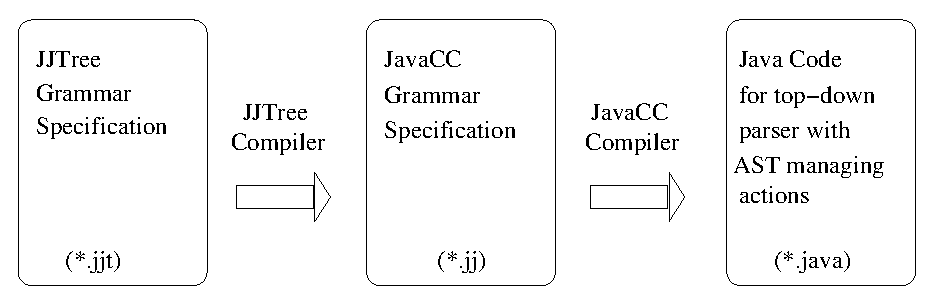
\includegraphics[scale=0.95]{linguaggio/dia/jjporc}
   \caption[Un parser con JJTree e JavaCC]{Generazione in due passi di un
   parser Java con JJTree e JavaCC.}
  \label{fig:lin:jjproc}
\end{center}
\end{figure}

A questo punto non ci rimane che mostrare come dalla sintassi di Tabella
\ref{tab:syntaxwsbpel} sia stata prodotta una grammatica EBNF che potesse
essere direttamente codificata nel linguaggio di specifica supportato da
JJTree.

Abbiamo già detto come, nonostante l'elevato supporto al lookahead fornito
da JavaCC, si sia scelto di mantenere la grammatica nella classe LL(1), questo
non tanto per motivi di efficienza, che per altro potrebbero essere sempre
rilevanti, ma per mantenere il più semplice possibile la definizione stessa
della grammatica che, per la ricchezza del linguaggio offerto da JJTree, tende
a complicarsi notevolmente. Inoltre ci è sembrato che i vincoli imposti dalla
classe LL(1) non appesantissero la sintassi ma che anzi contribuissero a chiarirne
alcuni aspetti, come per esempio la distinzione fra la definizione di processo
e le istanze pronte per essere eseguite (\emph{Ready to Run Instance}).

Come illustrato i passi da compiere sono quelli di eliminare la ricorsione
sinistra e i prefissi comuni nelle diverse parti destre associate al medesimo
non terminale. Di fatto tali criticità sono presenti nelle regole EBNF di tipo:

$$
\begin{array}{rcl}
\xs & ::= &
%\xb \!\sepgr\! 
\xs \xsucc\xs  
\!\sepgr\! \xs \xpar \xs 
\!\sepgr\! \xb \; ( \; + \; \xb  \; )^*  \\
 
\xd & ::= &  \xeng{\xI}{\xcorr} \!\sepgr\! \xd \, \xspar \xd
\end{array}
$$ 

In generale per risolvere il problema si può utilizzare l'approccio usato per
le espressione aritmetiche e introdurre i simboli terminali delle parentesi e
nuovi simboli non terminali e tramite questi riscrivere le regole nel
seguente modo:

$$
\begin{array}{rcccccl}
\xs 	& ::= & \x{sq}	& 	&&&\\
\x{sq} 	& ::= & \x{par} & (&  ; 	& \x{par} & )^+ \\
\x{par} & ::= & \x{pk} 	& (& \xpar & \x{pk}  & )^+ \\
\x{pk} 	& ::= & \x{ba}  & (& + 	& \x{ba}  & )^* \\
\x{ba}  & ::= & \xb 	& \sepgr & &( \xs ) \\
\\ 
\xd 	& ::= & \x{dep} & (& \xspar & \x{dep}  & )^+ \\
\x{dep} & ::= & \xeng{\xI}{\xcorr} 	& & & \\
\end{array}
$$ 

Si può banalmente vedere che tale grammatica è di classe LL(1) e quindi non
ambigua\footnote{Si può dimostrare che le grammatiche LL(1) non sono ambigue,
cioè essere in LL(1) è condizione sufficiente a garantire la non ambiguità di
una grammatica.}, infatti essa esplicita strutturalmente la precedenza
dell'operatore $;$ su $\xpar$ e la precedenza di quest'ultimo sull'operatore di
$+$. Il costo che si è dovuto pagare, oltre ad un aumento delle regole e dei
simboli non terminali, è la perdita di chiarezza e simmetria nella
grammatica che si traduce in una complicazione nella gestione
dell'albero sintattico in quanto dovranno essere implementate in maniera
specifica le azioni associate a ciascuna regola.

Tale approccio è stato utilizzato solo per la categoria sintattica dei
deployment $\xd$ ma non per quella delle attività strutturate $\xs$. Per
queste ultime si è preferito un approccio che aggiungendo dei nuovi simboli
terminali (usati come delimitatori di blocco) permettesse di ottenere un
grammatica LL(1) mantenendo una certa simmetria nella definizione e facilitando
la gestione dell'albero sintattico.

Quello che abbiamo fatto è stato di introdurre per ogni operatore un coppia di
simboli terminali che delimitasse la rispettiva attività
strutturale, di fatto vengono introdotte regole del seguente tipo:

$$
\begin{array}{rcl}
Activity &	::= & 	BasicActivity \hspace{0.2cm}| \hspace{0.2cm}SequenceActivity
\hspace{0.2cm}|\hspace{0.2cm} Scope \hspace{0.2cm}| \\ 
&& FlowActivity \hspace{0.2cm}| \hspace{0.2cm}PickActivity \hspace{0.2cm}|\\
&&ConditionalActivity \hspace{0.2cm}| \hspace{0.2cm}IterationActivity \\
\ldots\\ 
SequenceActivity &	::= & \verb#"seq"# \hspace{0.2cm} Activity \hspace{0.2cm} (
\verb#";"#  \hspace{0.2cm} ( Activity )? \hspace{0.2cm} )* \hspace{0.2cm}
\verb#"qes"# \\
 
FlowActivity &	::=  &	\verb#"flw"#  \hspace{0.2cm} Activity \hspace{0.2cm} (
\verb#"|"#  \hspace{0.2cm} Activity \hspace{0.2cm})+ \hspace{0.2cm}
\verb#"wlf"# \\

PickActivity &	::=  &	\verb#"pck"# \hspace{0.2cm} ReceiveActivity
\hspace{0.2cm} ( \verb#"+"#  \hspace{0.2cm} ReceiveActivity \hspace{0.2cm})+
\hspace{0.2cm} \verb#"kcp"# \\
\end{array}
$$

\begin{table}
\begin{center}
\begin{tabular}{|r|c|c|}
\hline
 & Sintassi Blite & Sintassi Implementata \\
\hline
Sequenza & $\xs_1 \xsucc \xs_2 \ldots \xsucc \xs_n $ & $seq \; \xs_1 \xsucc
\xs_2 \ldots \xsucc \xs_n \; qes$ \\
\hline
Parallelismo & $\xs_1 \xpar \xs_2 \ldots \xpar \xs_n $ & $flw \; \xs_1 \xpar
\xs_2 \ldots \xpar \xs_n \; wlf$ \\
\hline
Scelta Esterna & $\xrec{}{}{}_1 + \xrec{}{}{}_2
\ldots + \xrec{}{}{}_n $ & $pck \; \xrec{}{}{}_1 + 
\xrec{}{}{}_2 \ldots + \xrec{}{}{}_n \; kcp$ \\
\hline
\end{tabular}
\caption[Delimitatori di blocco per le attività strutturate]{Utilizzo dei
delimitatori di blocco per le attività strutturate con operatori binari.}
\label{tab:blokmarks}
\end{center}
\end{table}

In ogni modo la motivazione che ci ha spinto maggiormente a propendere per
l'utilizzo dei delimitatori, è stata quella di avere una sintassi il più chiara
possibile e che non lasciasse a regole implicite la determinazione delle
precedenze fra gli operatori. In questo modo il codice stesso espliciterà tutte le
relazioni di sequenzialità fra le diverse attività strutturate, e l'utilizzatore non sarà
obbligato a ricordare le regole di priorità fra i vari costrutti.

In Figura \ref{fig:lin:blt1} è rappresentato, nella sintassi
da noi implementata, il programma corrispondente al termine seguente:

$$
\begin{array}{rl}
\xeng{
(
	\xrec{\arr{"auction"} }{\x{seller}}{\arr{pid, seller}}
	\xpar
	\xrec{\arr{"auction"} }{\x{buyer}}{\arr{pid, buyer}} 
)
\\
\xsucc 
\xinv{\arr{seller} }{\x{ok}}{\arr{pid, buyer}}
\xsucc
\xinv{\arr{buyer} }{\x{ok}}{\arr{pid, seller}}
}{(pid)}
\end{array}
$$

A scapito di una maggiore compattezza si è guadagnato in chiarezza. Inoltre
le tecnologie attuali offrono un alto grado di assistenza all'editing del
codice, per cui sarà facilmente implementabile un editor che possa supportare
l'utente nella scrittura dei costrutti previsti dalla nostra grammatica.
\\

\begin{figure}[!t]
\begin{center}
  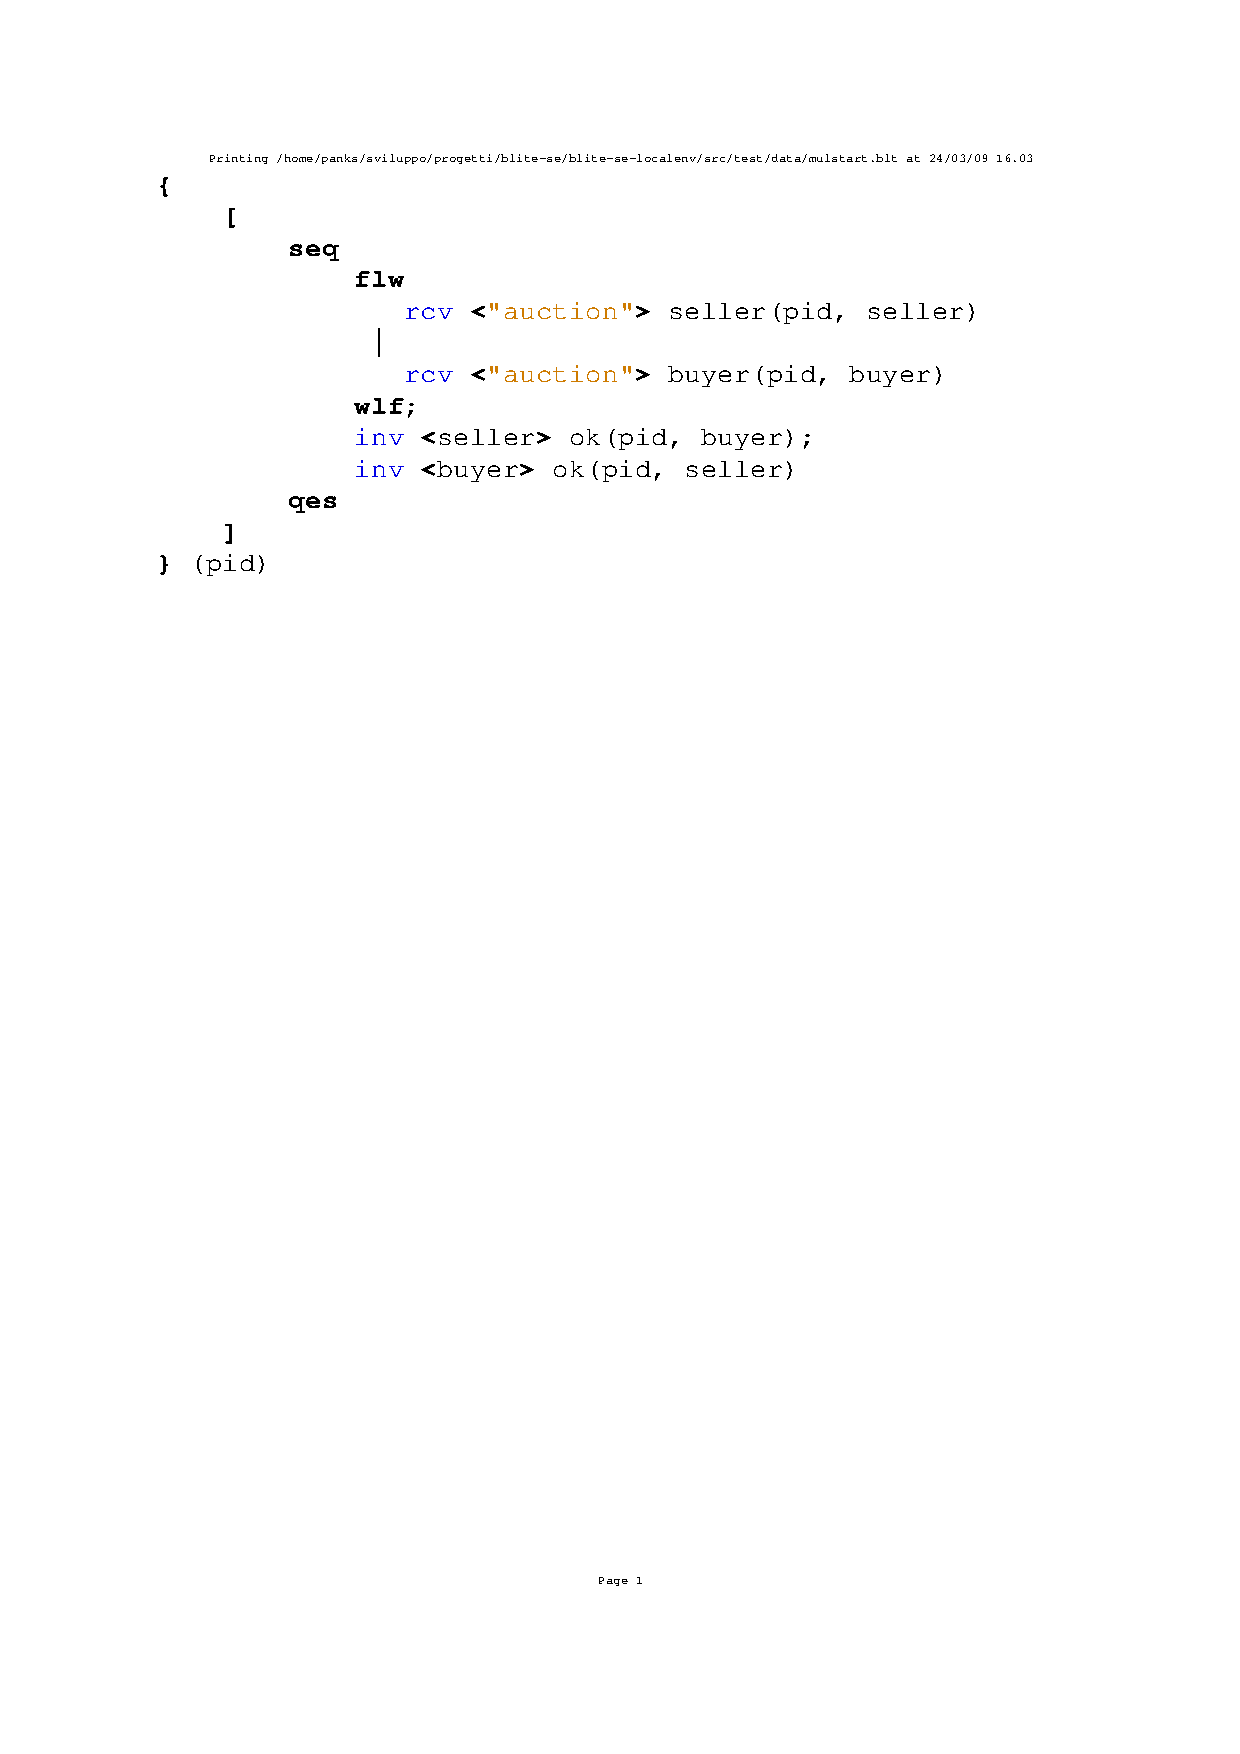
\includegraphics[scale=0.80,clip]{linguaggio/dia/blt1}
   \caption[Codice Blite, esempio delimitatori di blocco]{Esempio di programma
   Blite con la sintassi dei delimitatori di blocco per le attività struturate.}
  \label{fig:lin:blt1}
\end{center}
\end{figure}


Un altro aspetto da considerare nella sintassi di Tabella \ref{tab:syntaxwsbpel}
è quello legato alla definizione dei termini \textit{Services}, tramite la
regola:
$$
\begin{array}{rcccl}
\textit{(Services)} & \xI & ::= &
\xproc{\xsa}{\xh_f} \sepgr
\xinst{\xsigma}{\xs} \sepgr
\xinst{\xsigma}{\xs} \xmid \xI & \textrm{definition, instance,
multiset}
\end{array}
$$ 

La parte destra \emph{instance} ha la funzionalità di rappresentare le istanze in
fase di esecuzione con uno stato di memoria ($\xinst{\xsigma}{\xs}$), ma anche di
dare la possibilità di definire, e quindi di rendere immediatamente disponibili
nei deployment, istanze di processo che sono già pronte per andare in
esecuzione, senza dover ricevere messaggi di attivazione.
Tali definizioni sono qui identificate con l'espressione
\emph{Ready-to-Run Instance}.

Nel linguaggio da noi implementato si è voluto mantenere quest'ultima
possibilità in quanto ci sembra molto utile, nell'ottica di voler fornire uno
strumento per la prototipizzazione, avere un meccanismo, integrato nel
formalismo, che possa permettere di avviare i processi\footnote{Si fa osservare
che in BPEL tale possibilità non è presente. Il formalismo di BPEL prevede
solamente la definizione di processi che interagiscono con il mondo esterno
esclusivamente attraverso le porte dei servizi web. L'unico modo di avviare le
istanze di processo è quello di inviare un messaggio ad una start activity tramite l'uso
di una tecnologia alternativa. Per esempio un'applicazione Java può fare un
invocazione ad una porta di una start activity e istanziare il processo BPEL}.

I tal senso si vuole dare la possibilità all'utente di poter definire dei
deployment del tipo: 
$$
\xeng{
\xs_1 \xmid \ldots \xmid \xs_n \xmid
\xproc{\xsa}{\xh_f}  
}{\xcorr}
$$
in cui è presente la definizione di processo  $\xproc{\xsa}{\xh_f}$ e $n$
ready-to-run instance. Per non appesantire ulteriormente la sintassi, il
linguaggio da noi implementato non prevede un formalismo specifico per la definizione della funzione di stato $\xsigma$ nelle ready to run instance, anche perché lo stato
iniziale di tali istanze può essere definito semplicemente con attività di
assegnamento. Di fatto quindi la distinzione fra le ready-to-run instance e la
definizione di processo sta semplicemente nel fatto che quest'ultima deve
obbligatoriamente avere la struttura  $\xproc{\xsa}{\xh_f}$, mentre le prime
possono essere generiche attività strutturate. Nel caso quindi queste siano dei
contesti, devono sempre esplicitare il compensation handler
($\xscopefc{\xsa}{\xh_f}{\xh_c}$) per essere distinguibili dalle definizioni.

Si capisce come limitandosi a tale sintassi non sia possibile prescindere
dall'eseguire lookahead sintattico per distinguere le definizioni dalle
ready-to-run instance, in quanto in generale tali termini possono avere prefissi comuni del tipo $"[\xs \bullet \xh_f"$. Anche in questo caso si è preferito
introdurre un nuovo terminale che preposto alle ready-to-run instance le
rendesse immediatamente riconoscibili, ottenendo quindi una grammatica LL(1)
e aumentando la leggibilità dei programmi.

In pratica si è introdotto il simbolo $\verb#::#$ e nella grammatica si sono
definite le seguenti regole per la definizione della categoria sintattica
\emph{Service}:

$$
\begin{array}{rcl}
Service & ::= &  ServiceDef \hspace{0.2cm} | \hspace{0.2cm} ( ServiceInstance
\hspace{0.2cm}( \verb#","# \hspace{0.2cm} Service  )? \hspace{0.2cm} )  \\ 

ServiceInstance & ::= &  \verb#"::"# \hspace{0.2cm} Activity \\
 
ServiceDef & ::= & \verb#"["# \hspace{0.2cm} StartActivity \hspace{0.2cm} (
\verb#"fh:"# \hspace{0.2cm} Activity )? \hspace{0.2cm} \verb#"]"# \\

\end{array}
$$

Usando un prefisso per distinguere le ready to run instance dalle
definizioni di processo, cade l'obbligatorietà di avere sempre un compensation
handler nelle scope activity generiche, per cui queste ultime potranno essere
definite tramite la seguente regola in cui risultano opzionali sia la
definizione del compensation che del fault handler:

$$
\begin{array}{rcl}
Scope & ::= & \verb#"["# \hspace{0.2cm} Activity \hspace{0.2cm} (
\verb#"fh:"# \hspace{0.2cm} Activity \hspace{0.2cm})? \hspace{0.2cm}(
\verb#"ch:"# \hspace{0.2cm}Activity \hspace{0.2cm})?\hspace{0.2cm} \verb#"]"#
\end{array}
$$

I simboli tipografici $\bullet$ e $\star$ sono stati sostituiti rispettivamente
dalle scritture \verb#fh:# e \verb#ch:# e si assume che un contesto che non
definisca gli handler, implicitamente preveda l'attività $\xthr$ come fault
handler e l'attività $\xskip$ come compensation handler. In pratica si assume
che \label{defHandelr}

$$
\x{[a]} = \xscopefc{\xs}{\xthr}{\xskip}
$$

\begin{figure}[!t]
\begin{center}
  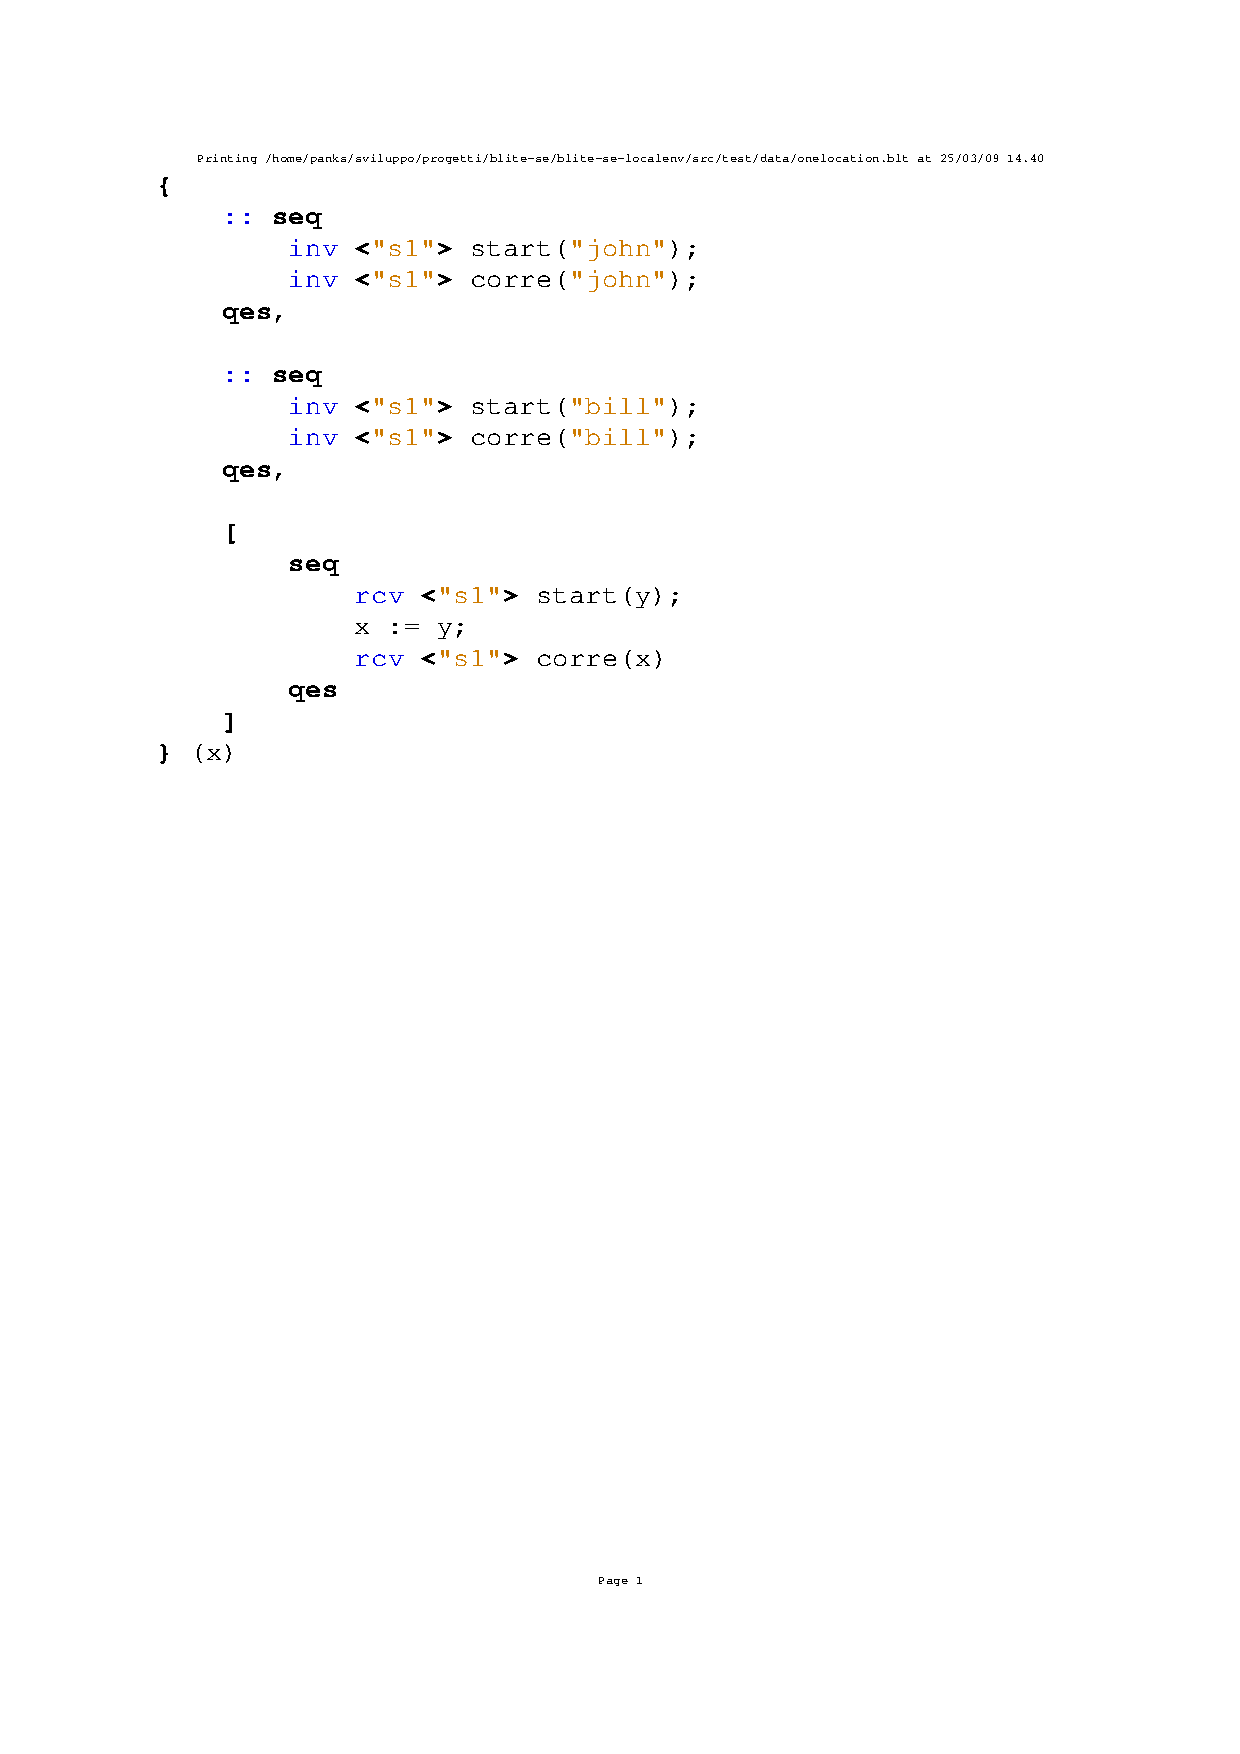
\includegraphics[scale=0.80,clip]{linguaggio/dia/blt2}
   \caption[Codice Blite, esempio ready to run instance]{Esempio di programma
   Blite con un deployment in cui è presente una definizione di processo e due
   istanze ready-to-run.}
  \label{fig:lin:blt2}
\end{center}
\end{figure}

In Figura \ref{fig:lin:blt2} è riportato un frammento di codice Blite in cui è
definito un deployment con una definizione di processo e due istanze pronte per
essere eseguite.

Con i simboli terminali introdotti tutte le attività strutturate risultano
avere un prefisso caratterizzante per cui nelle regole di Tabella
\ref{tab:syntaxwsbpel} che definiscono l'attività condizionata e l'iterazione  

$$
\begin{array}{rccccl}
\textit{(Structured activities)} & \xs & ::= & \ldots  &
\xif{\xe}{\xs_1}{\xs_2} \!\sepgr\! \xwhile{\xe}{\xs} & \ldots
\end{array}
$$ 
possono essere eliminati i delimitatori di blocco $\{\cdot \}$ e definire le
seguenti regole: $$
\begin{array}{rcl}
ConditionalActivity & ::= & \verb#"if"# \hspace{0.2cm} \verb#"("#
\hspace{0.2cm} Expression \hspace{0.2cm} \verb#")"#  \hspace{0.2cm} Activity
\hspace{0.2cm} Activity \\

IterationActivity & ::= & \verb#"while"# \hspace{0.2cm} \verb#"("#
\hspace{0.2cm} Expression \hspace{0.2cm} \verb#")"#  \hspace{0.2cm} Activity \\
\end{array}
$$

Si deve osservare che dopo la scelta interna devono essere sempre esplicitate
(eventualmente con $\xskip$) entrambe le attività che realizzano le
alternative.
\\

In appendice è riportato il lessico e in notazione EBNF la grammatica completa
che definisce il linguaggio da noi implementato. In essa sono specificati
i tipi supportati (attualmente stringhe, numeri -interi e decimali- e booleani)
e la sintassi delle espressioni logiche e aritmetiche.

%%%%%%%%%%%%%%%%%%%%%%%%%%%%%%%%%%%%%%%%%%%%%%%%%%%%%%%%%%%%%%%%%%%%%%%%%%%%%%%%
% SEMANTICA CONCRETA
\section{Alcune osservazioni sulla semantica della correlazione}
\label{sec:semcor}

La sematica presentata in Sezione \ref{sec:blite} descrive il comportamento dei
programmi Blite in modo molto elgante e sintetico. Il nostro obbiettivo è stato
quello di creare un motore capace di eseguire i programmi producendo un
comportamento equivalente a quello specificato nel rispetto di specifiche
tecniche che tenessero conto il più possibile di problematiche di efficenza,
scalabilità e requisiti di memoria.

Come vedremo nel capitolo seguente alla base dell'architettura software
realizzata, ci sono due componenti fondamentali:

\begin{itemize}
  \item Un oggetto software chiamato \icode{ProcessManger}, che, data una   
  precisa definizione di processo, ha la rasponsabilità di creare le istanze
  e di metterle in esecuzione. Inolte, tale oggetto ha la responsabilità di
  gestire - memorizzandoli in opportune strutture dati- i messaggi indirizzati alle porte
  della propria definizione.
  \item Un insieme di thread, \icode{ThreadPool}, che eseguono concorrentemente
  le varie istanze di processo e i flussi paralleli che si generano in esse.
\end{itemize}

Gli aspetti più critici nella realizzazione del compoeramento specificato
sono quelli di attribuire i messaggi alle diverse istanze e di discriminare se
l'arrivo di un messaggio debba produrre o meno la creazione di una nuova
istanza (regole \rulelabel{$\x{com}$} e \rulelabel{$\x{new}$} di Tabella
\ref{tab:deploySOS}).

In riferimento alla prima problematica la sematica definisce un ordinamento fra
tutte le istanze che \emph{contemporaneamente} attivano una ricezione su una
determinata porta\footnote{Con il termine porta si intende la coppia $\langle
\texttt{service-name}, \texttt{operation-name} \rangle$, essa indentifica
univocamente una funzionalità operazione nell'interfaccia associata ad una
definizione di processo.}, ed in base a tale ordinamento si stabilisce
l'attribuzione del messaggio. Di fatto in una architettura come la nostra, che
usa una tecnologia di \emph{multithreading} per realizzare la non sequezialità
specificata dalla semantica di Blite, non ha molto senso parlare di attività di
ricezione contemporaneamente attivie su una porta. In pratica quando il
flusso di escuzione di una istanza arriva ad eseguire un ricezione su una
determinata porta si deve poter decidere se un messaggio associato alla porta è
destinabile a tale istanza solamente in base allo stato attuale dell'istanza
stessa.


Sempificando, per valutare se un messaggio possa essere attribuito ad una
insanza che esegue l'operazione
$\xrec{\arr{\x{p}}}{\x{o}}{\bar{\xx}}$, si può pensare di attuare la seguente
procedura:

\begin{verbatim}
               m := null
               for each v in { messages on <p,o>} 
                   if corr(x, v) 
                      m := v
                      break iteration
    
               if m is null start wainting on <p,o>
               else 
                   consume m
                   continue-execution
\end{verbatim}
in cui ``\texttt{messages on <p,o>}'' identifica tutti i
messaggi ricevuti sulla porta \texttt{<p,o>} e la funzione \texttt{corr(x, v)},
che restituisce un valore booleano, valuta se il messaggio \texttt{v} può essere correlato all'istanza in
base ai parametri attuali \texttt{x}, allo stato dell'istanza e al correlation
set definito dal progrmmatore.

In pratica tale funzione può essere ricavata, in riferimento alla funzione
$\xxnewmatch{\xcorr}{\xsigma}{\bar{\xx}}{\bar{\xv}}$ definita in Sezione
\ref{pag:match}, nel seguente modo:
$$
\begin{array}{c}
\x{corr}(\xcorr, \xsigma, \xx, \xv	) =
\left\{
\begin{array}{l@{\hspace{2ex}}l}
\\[-.50cm]
false & \textrm{se}\ \xx \in \xcorr \, \wedge \, \xx \in \xdom{\xsigma} \in
\xcorr\ \, \wedge \, \xv \neq \xsigma(\xx)
\\[-.05cm] true & \textrm{altrimenti} \\
\end{array}
\right.
\\[.7cm]
%\xxnewmatch{\xcorr}{\xsigma}{\xv}{\xv} =
%\emptyset \qquad
\x{corr}(\xcorr, \xsigma, \arr{}, \arr{}) =
true
\\[.7cm]
\prooftree
\x{corr}(\xcorr, \xsigma, \xx_1, \xv_1) = b'
\quad
\x{corr}(\xcorr, \xsigma, \bar{\xx}_2, \bar{\xv}_2) = b''
\justifies \
\x{corr}(\xcorr, \xsigma, (\xx_1,\bar{\xx}_2), (\xv_1,\bar{\xv}_2)) =
b' \wedge b''
\endprooftree
\\[.7cm]
\end{array}
$$
in cui $\xsigma$ rappresenta lo stato di momoria associato all'istanza e
$\xcorr$ il correlation set associato alla definizione di processo da cui
l'istanza è ricavata.

Questa strategia risolve il problema della correlazione dei messaggi con
le istanze di processo, producedendo un comportamento equivalente ad quello
specificato dalla sematica formale di Blite. Si fa notare infatti che
la sematica non risolve più conflitti rispetto alla nostra implemetazione in
quanto la regola \rulelabel{$\x{pass}$} porta ad attivare in modo indeterminato
le attività di ricezione delle diverse istanze.

I concetti di \emph{grado di definizione} e di ordinamento delle istanze
rispetto alla possibilità di consumare messaggi in arrivo, introdotti dalla
semantica di Blite, risultano invece determinanti per descriminare quando si
deve creare una nuova istanza, e in particolare per realizzare le \emph{multiple
start activity}.

Le multiple start activity, sono attività di inzio istanza del tipo:
$$
	\xrec{\plrec_1}{\xo_1}{\bar{\xx_1}} \xsucc \xs_1 
	\, \xpar \, 
	\xrec{\plrec_2}{\xo_2}{\bar{\xx_2}} \xsucc \xs_2
$$
in cui la start activity è costituita dalla composizione parallela di più
ricezioni. 

La specifica BPEL afferma, anche se in maniera non molto esplicita\footnote{Per
esempio, nella specifica di BEPEL4WS 1.1 \cite{BPEL11Spec} il comportamento
associato alle multiple start activity era addirittura descritto semplicemente
con un esempio (sezione 1.6).}, che nel caso delle multiple start activity, la
correlazione di un messaggio ad una istanza abbia precedenza sulla creazione di
nuove istanze.

Questo comportamento è espresso alla perfezione dalla sematica di Blite che
determina in maniera univoca il comporatamento del seguente termine:\\
$$
\begin{array}{l}
\{
\xscopez{ (\xrec{\arr{\xp_1}}{\xo}{\arr{\xx}}
	 \xpar  \xrec{\arr{\xp_2}}{\xo}{\arr{\xx, \xz}}) 
	 \xsucc \xs}
\,\}_{\{\xx\}}
\\ 
\xspar 
\{
\xinst{\xenv{\assoc{\xy}{\xv}}}{\xinv{\arr{\xp_1}}{\xo}{\arr{\xy}}}
\}
\\
\xspar 
\{
\xinst{\xenv{\assoc{\xy_1}{\xv},
\assoc{\xy_2}{\xv'}}}{\xinv{\arr{\xp_2}}{\xo}{\arr{\xy_1, \xy_2}}}
\}
\end{array}
$$
$$
\begin{array}{c}
\ldots \bpelredarrow{} \ldots
\end{array}
$$
$$
\begin{array}{l}
\{
\xscopez{ (\xrec{\arr{\xp_1}}{\xo}{\arr{\xx}}
	 \xpar  \xrec{\arr{\xp_2}}{\xo}{\arr{\xx, \xz}}) 
	 \xsucc \xs}
\, , 
\xinst{\xenv{\assoc{\xx}{\xv}}}{ 
	\xscopez{\xrec{\arr{\xp_2}}{\xo}{\arr{\xx, \xz}})
	\xsucc \xs }} 
\}_{\{\xx\}}
\\
\xspar 
\{
\xinst{\xenv{\assoc{\xy_1}{\xv},
\assoc{\xy_2}{\xv'}}}{\xinv{\arr{\xp_2}}{\xo}{\arr{\xy_1, \xy_2}}}
\}
\end{array}
$$
$$
\begin{array}{c}
\ldots \bpelredarrow{} \ldots
\end{array}
$$
$$
\begin{array}{l}
\{
\xscopez{ (\xrec{\arr{\xp_1}}{\xo}{\arr{\xx}}
	 \xpar  \xrec{\arr{\xp_2}}{\xo}{\arr{\xx, \xz}}) 
	 \xsucc \xs}
\, , 
\xinst{\xenv{\assoc{\xx}{\xv}, \assoc{\xz}{\xv'}}}{ 
\xscopez{\xs} } 
\}_{\{\xx\}}
\end{array}
$$
in cui dalla definizione viene creata un'unica istanza di processo.

Nella nostra implemetazione il \icode{ProcessManager}, nel momento in cui arriva
un nuovo messaggio deve poter decidere se creare una nuova istanza o meno in
base alle informazioni di cui dispone in quel momento.

In generale si potrebbe pensare di risolvere semplicemente il problema a livello
sintattico rendendo distinguibili le porte di
ricezione su cui vengono create le istanze (\emph{create port}). In pratica si
potrebbe semplicemete dire che un messaggio su una porta che è utilizzata in
una start activity porta sempre alla creazione di una nuova istanza, lasciando
al programmatore la responsabilità di non riutilizzare tali porte per
effettuare la correlazione (in quanto tale correlazione mai si realizzarebbe).

\`E ovvio che questa tecnica, non permetta di realizzare le multiple
start activity, in cui una porta è contemporaneamente di creazione e di possibile
correlazione, e in generale produca comportamenti non coformi alla sematica
specificata.
\\

Per ottenere il comportamento specificato dalla semantica di
Blite, compreso il caso delle multiple start activity, si deve fare in modo
che il \icode{ProcessManager}, all'arrivo di un messaggio
$\xmsg{{\xp}}{\xo}{\bar{\xv}}$,  attui la seguente procedura:
\begin{verbatim}
On a new message v:

               put v in { messages on <p,o> } 
               for each 'rcv <p> o x' wainting on <p,o>
                   if cor(x, v) goto continue

               if <p,o> is a create port 
                   create a new instance i
                   start i
                   wait until all start rcv of i are activated
               
   continue:   manage next message 
\end{verbatim}

In pratica viene creata una nuova istanza solo se il messaggio è indirizzato
a una porta di creazione, e non c'è nessuna attività di
ricezione (fra tutte le varie istanze) in attesa su tale porta che possa
correlare con il messaggio. Inoltre si fa notare come la procedura di gestione
dei nuovi messaggi, dopo aver creato un nuova istanza e averla messa in
escuzione, attenda che tutte le sue start activity di ricezzione si siano
attivate, cioè si siano registrate come in attesa sulle rispettive porte o
abbiamo consumato qualche messaggio. Solo dopo questo tornerà a gestire altri
messaggi in arrivo. In questo modo si realizza l'atomicità del passo descritto dalle regola (new),
in cui in un solo posso si crea un nuova istanza, si attivano le attività di
ricezione. Così si realizza la semantica delle multiple start activity secondo
cui la correlazione ha priorità sulla creazione di istanze.

Queste osservazioni risulteranno più chiare dopo ever letto il Capitolo 4 in cui
verrà presentata l'architettura e il modello di esecuzione dell'Engine. In questa
fase sono state presentate per illustrare come il processo di interpretazione
della sematica risulti particolarmente delicato e in come in presenza di una
architettura multithreading siano necessari algoritmi e strutture dati non
banalmente deducibili dalla semantica stessa. Inoltre è chiaro come risultino
indispensabili meccanismi di sincronizzazione fra i vari thread
eseguiti concorrentemente.


 


